%!LW recipe=latexmk-xelatex
\documentclass[compress]{beamer}

\usetheme[block=fill]{metropolis}

\usepackage{graphicx} % Allows including images
\usepackage{amsmath,amsfonts,amsthm,amssymb}
\usepackage{color}
\usepackage{xcolor,cancel}
\usepackage[shortlabels]{enumitem}
\setitemize{label=\usebeamerfont*{itemize item}%
	\usebeamercolor[fg]{itemize item}
	\usebeamertemplate{itemize item}}
\definecolor{mDarkBrown}{HTML}{604c38}
\definecolor{mDarkTeal}{HTML}{23373b}
\definecolor{mLightBrown}{HTML}{EB811B}
\definecolor{mMediumBrown}{HTML}{C87A2F}
\definecolor{mygreen}{HTML}{98C2B9}
\definecolor{myyellow}{HTML}{DFD79C}
\definecolor{myblue}{HTML}{8CA7CC}
\definecolor{kern}{HTML}{8CC2B7}


\usepackage{float}
\usepackage{framed}
\usepackage{epsfig}
\usepackage{graphicx}
\usepackage{subcaption}
\usepackage{ulem}
\usepackage{hhline}
\usepackage{multirow}
\usepackage{comment}   
\usepackage{bbm}
\usepackage{tikz}   
\def\Put(#1,#2)#3{\leavevmode\makebox(0,0){\put(#1,#2){#3}}}
\newcommand*\mystrut[1]{\vrule width0pt height0pt depth#1\relax}
\newcommand{\eqdef}{\mathbin{\stackrel{\rm def}{=}}}


\newcommand{\bs}[1]{\boldsymbol{#1}}
\newcommand{\bv}[1]{\mathbf{#1}}
\newcommand{\R}{\mathbb{R}}
\newcommand{\E}{\mathbb{E}}

\DeclareMathOperator*{\argmin}{arg\,min}
\DeclareMathOperator*{\argmax}{arg\,max}
\DeclareMathOperator{\nnz}{nnz}
\DeclareMathOperator{\Var}{Var}
\DeclareMathOperator{\diag}{diag}
\DeclareMathOperator{\sinc}{sinc}
\DeclareMathOperator{\sign}{sign}
\DeclareMathOperator{\dist}{dist}
\DeclareMathOperator{\mv}{mv}
\DeclareMathOperator{\sgn}{sgn}
\DeclareMathOperator{\step}{step}
\DeclareMathOperator{\gap}{gap}
\DeclareMathOperator{\poly}{poly}
\DeclareMathOperator{\tr}{tr}
\DeclareMathOperator{\orth}{orth}
\newcommand{\norm}[1]{\|#1\|}
\captionsetup[subfigure]{labelformat=empty}
\captionsetup[figure]{labelformat=empty}
\DeclareMathOperator*{\lmin}{\lambda_{min}}
\DeclareMathOperator*{\lmax}{\lambda_{max}}

\newcommand{\specialcell}[2][c]{%
  \begin{tabular}[#1]{@{}c@{}}#2\end{tabular}}
\newcommand{\specialcellleft}[2][c]{%
\begin{tabular}[#1]{@{}l@{}}#2\end{tabular}
}

\newtheorem{claim}[theorem]{Claim}

\usepackage{tabstackengine}
\stackMath


%----------------------------------------------------------------------------------------
%	TITLE PAGE
%----------------------------------------------------------------------------------------

\title{CS-GY 6763: Lecture 6 \\ Gradient Descent and Projected Gradient Descent}
\author{NYU Tandon School of Engineering, Prof. Christopher Musco}
\date{}

\begin{document}

\begin{frame}
	\titlepage 
\end{frame}

\metroset{titleformat=smallcaps}

\begin{frame}
	\frametitle{administrative}
	\begin{itemize}
		\item Homework 3 due on Monday.
		\item Exam on Friday. 1 hour 15 minutes, cheat sheet allowed. 
	\end{itemize}
\end{frame}

\begin{frame}[standout]
	\begin{center}
		finish up lsh + near neighbor search
	\end{center}
\end{frame}

\begin{frame}
	\frametitle{locality sensitive hash functions}
	Let $h: \R^d \rightarrow \{1, \ldots, m\}$ be a random hash function. 
	
	We call $h$ \emph{locality sensitive} for similarity function $s(\bv{q},\bv{y})$ if $\Pr\left[h(\bv{q}) == h(\bv{y})\right]$ is:
	\begin{itemize}
		\item Higher when $\bv{q}$ and $\bv{y}$ are more similar, i.e. $s(\bv{q},\bv{y})$ is higher.
		\item Lower when $\bv{q}$ and $\bv{y}$ are more dissimilar, i.e. $s(\bv{q},\bv{y})$ is lower. 
	\end{itemize}
\begin{center}
	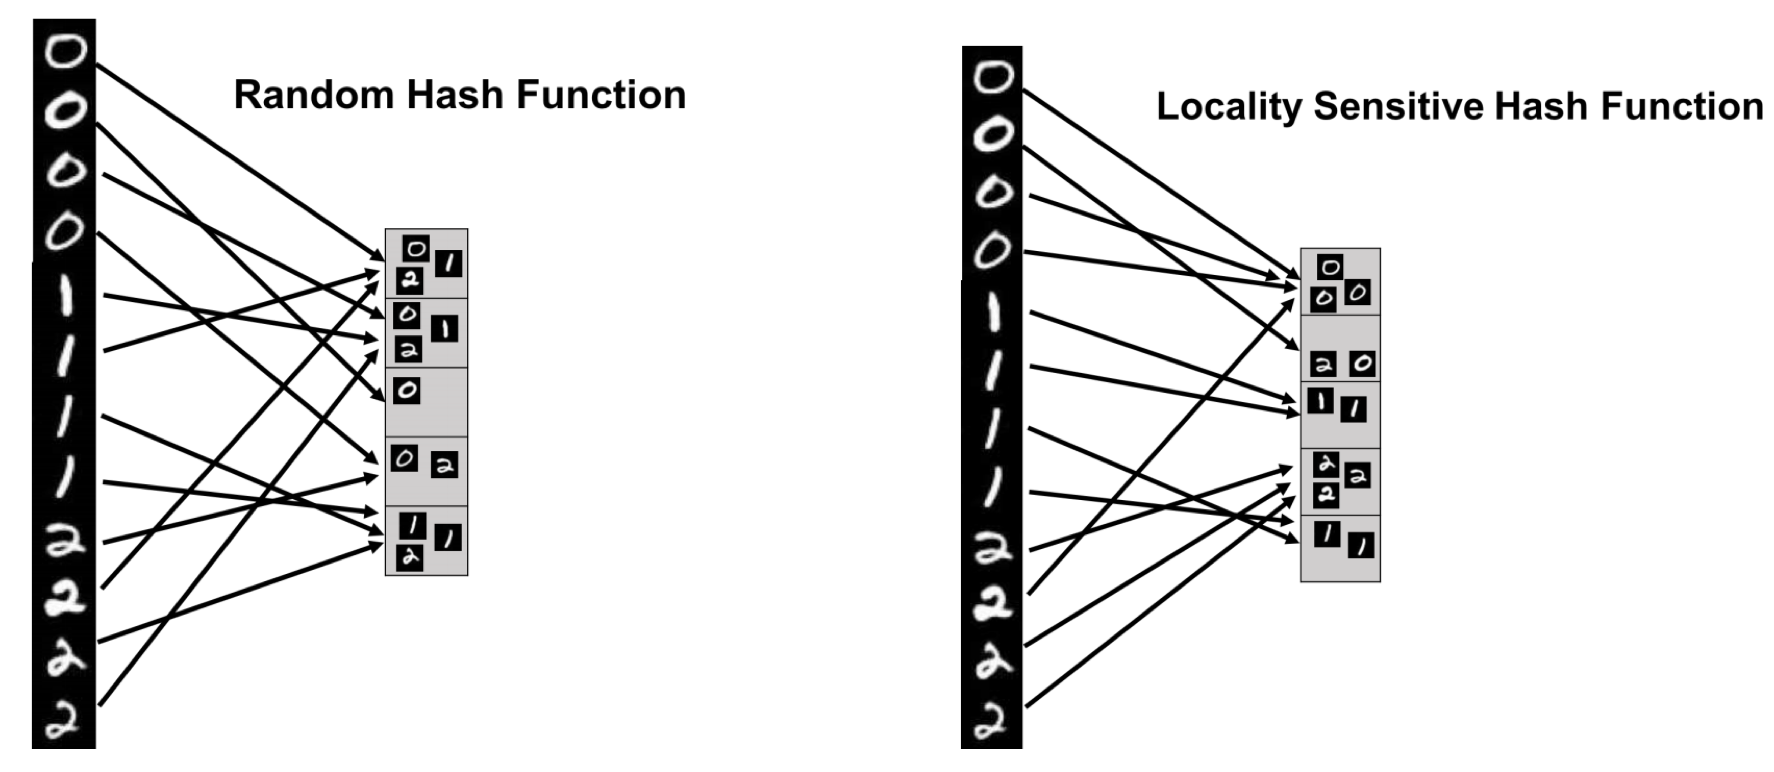
\includegraphics[width=.9\textwidth]{cam_lsh.png}
\end{center}
\end{frame}

\begin{frame}[t]
	\frametitle{nearest-neighbor search in practice}
	LSH is widely used in practice, but is starting to get replaced by other methods. Most of these are \emph{data dependent} in some way. 

	\textbf{Starting point:} Think of LSH as a randomized \emph{space-partitioning method}.
	\begin{center}
	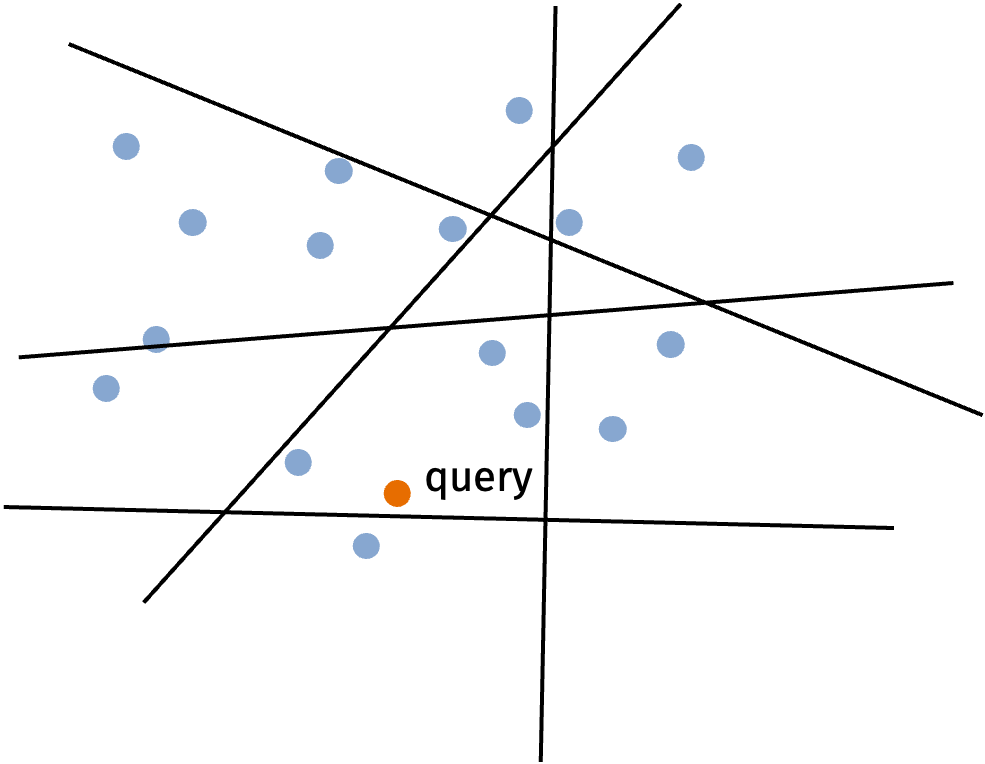
\includegraphics[width=.6\textwidth]{random_space_partition.png}
	\end{center}
\end{frame}

\begin{frame}[t]
	\frametitle{nearest-neighbor search in practice}
In practice, we can often get partitions with better \emph{margin} but partitioning in a data-dependent way. 

	\textbf{Common approach:} Split data using $k$-means clustering. 
	\begin{center}
	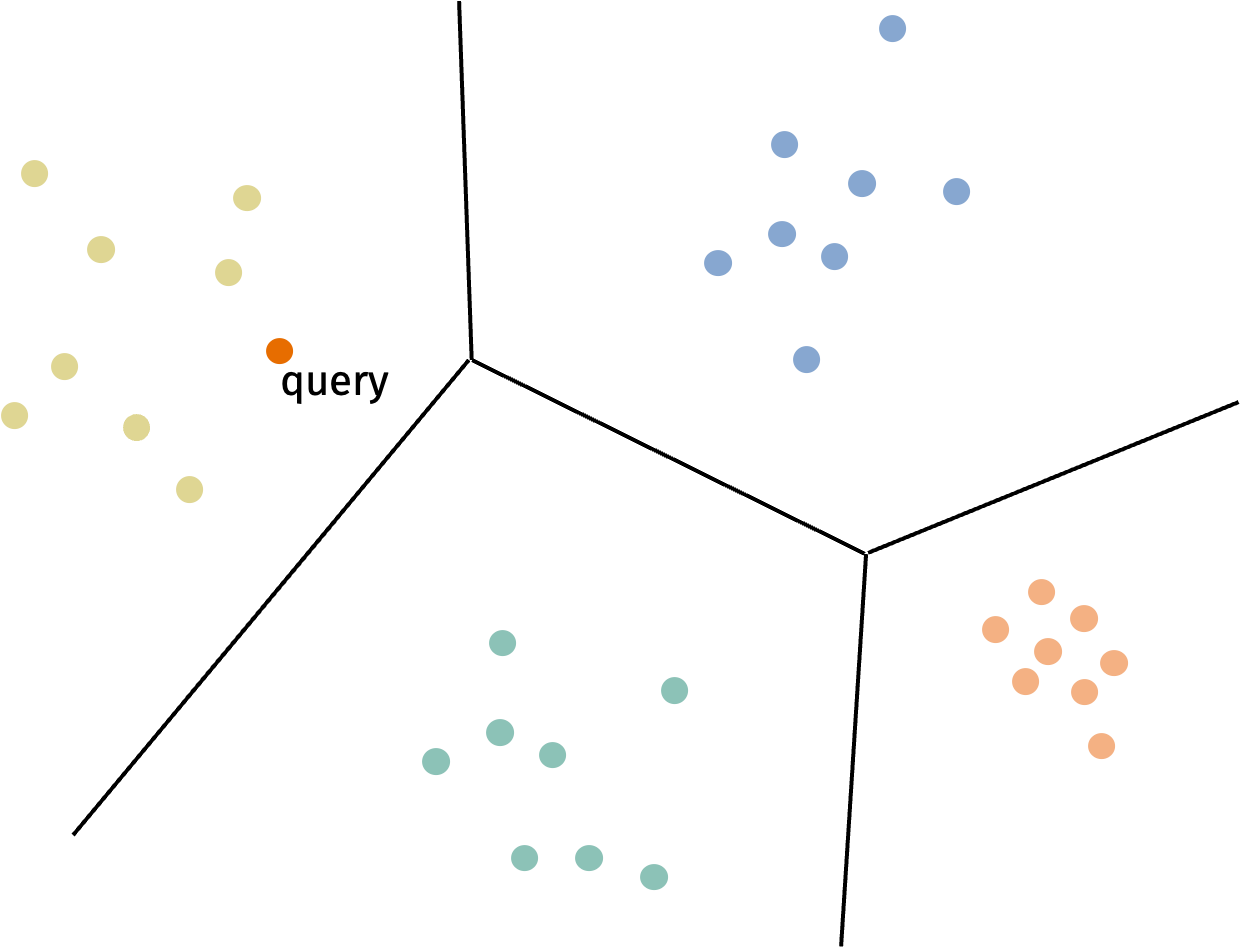
\includegraphics[width=.6\textwidth]{kmeans_1.png}
	\end{center}

\end{frame}

\begin{frame}[t]
	\frametitle{nearest-neighbor search in practice}
	\textbf{Common approach:} Split data using $k$-means clustering. 
	\begin{center}
	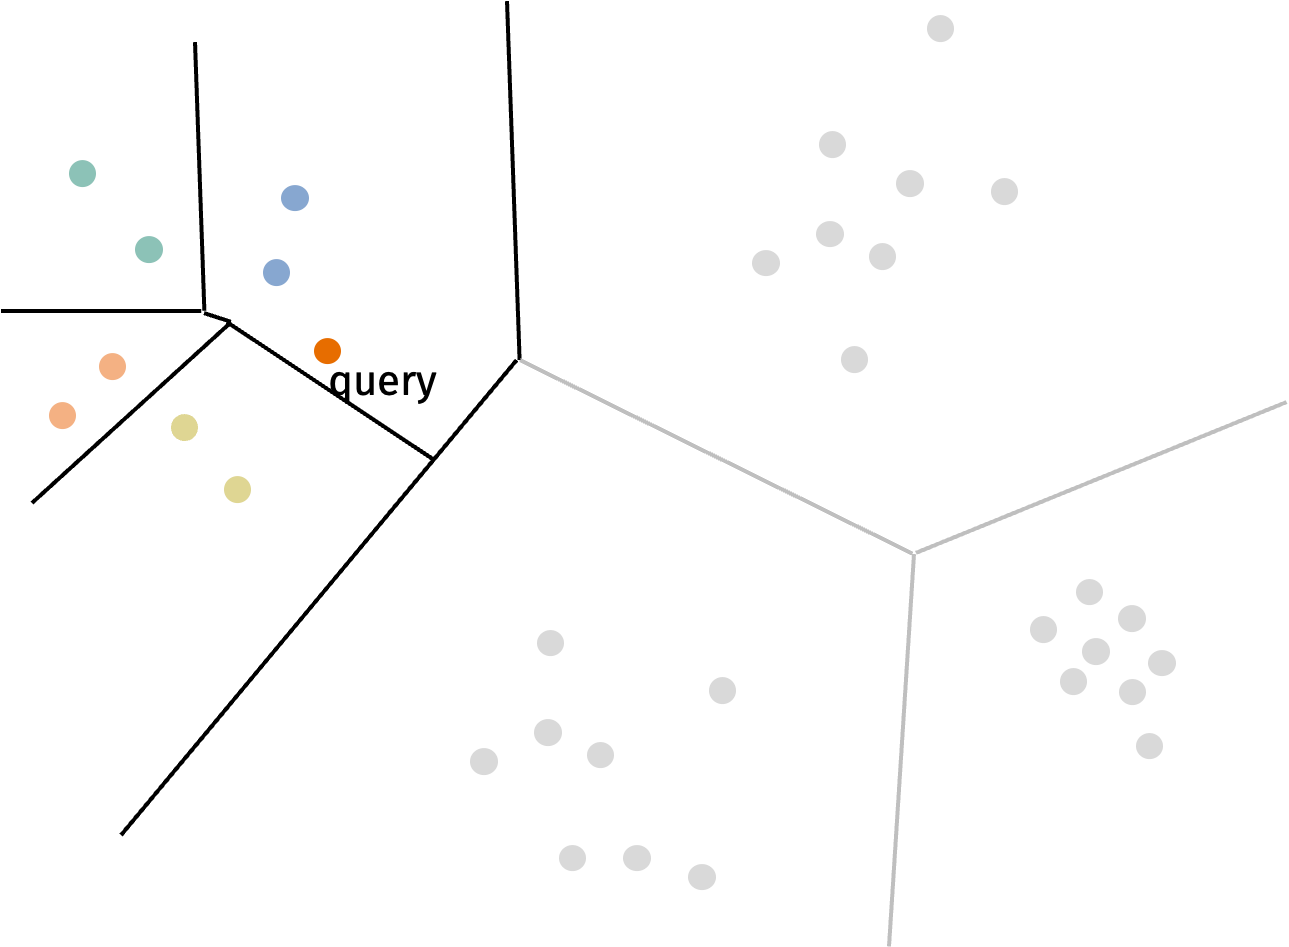
\includegraphics[width=.6\textwidth]{kmeans_2.png}
	\end{center}
	Main approach behind ``k-means tree'' and ``inverted file index'' based near-neighbor search methods like Meta's FAISS library and Google's SCANN. 
\end{frame}

\begin{frame}[t]
	\frametitle{nearest-neighbor search in practice}
	\textbf{New kid on the block:} Graph-based nearest neighbor search.
	\begin{center}
		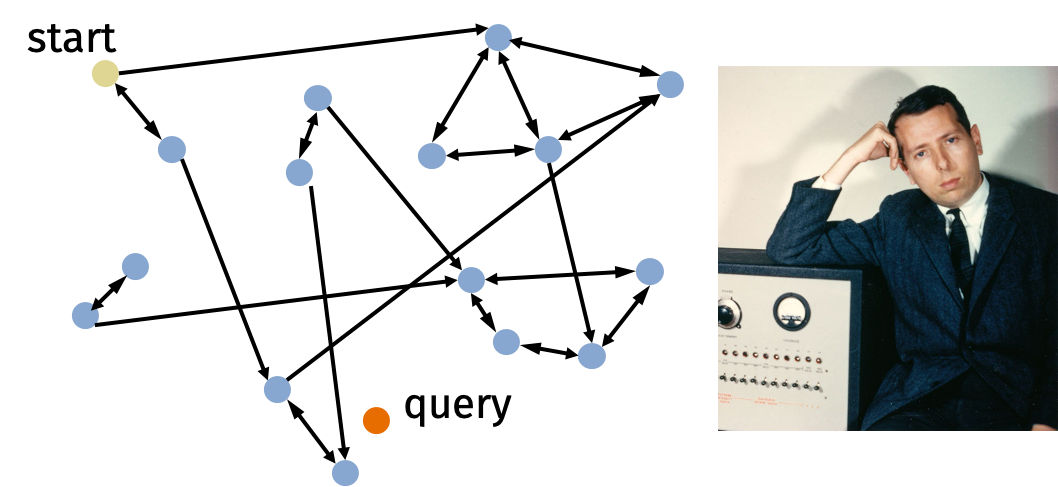
\includegraphics[width=\textwidth]{search_graph.png}
		\end{center}
Idea behind methods like NSG, HNSW, DiskANN, etc. Inspired by Milgram's famous ``small-world'' experiments from the 1960's. 
\end{frame}

\begin{frame}[t]
	\frametitle{open theory challenge}
	\textbf{Can we better explain the success of data-dependent nearest-neighbor search methods?}
	\begin{center}
		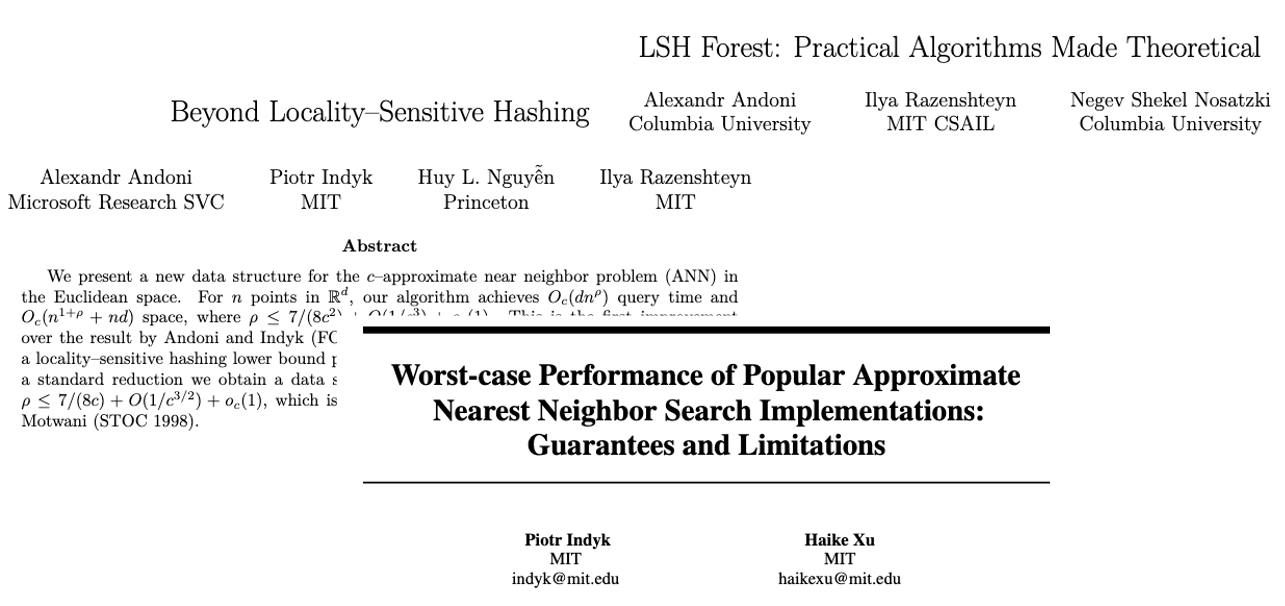
\includegraphics[width=\textwidth]{new_theory.png}
	\end{center}
\end{frame}


\begin{frame}[standout]
	\begin{center}
		optimization
	\end{center}
\end{frame}

\begin{frame}
	\frametitle{next unit: continuous optimization}
	Have some function $f : \R^d \rightarrow \R$. Want to find ${\bv{x}}^*$ such that:
	\begin{align*}
		f({\bv{x}}^*) = \min_{\bv{x}} f(\bv{x}).
	\end{align*}
	Or at least $\hat{\bv{x}}$ which is close to a minimum. E.g. $$f(\hat{\bv{x}}) \leq \min_{\bv{x}} f(\bv{x}) + \epsilon.$$
	
	Often we have some additional constraints:
	\begin{itemize}
		\item $\bv{x} > 0$.
		\item $\|\bv{x}\|_2 \leq R$, $\|\bv{x}\|_1 \leq R$.
		\item $\bv{a}^T\bv{x} = c$.
	\end{itemize}
\end{frame}

\begin{frame}
	\frametitle{continuous optimization}
	\textbf{Dimension $d = 1$:}
	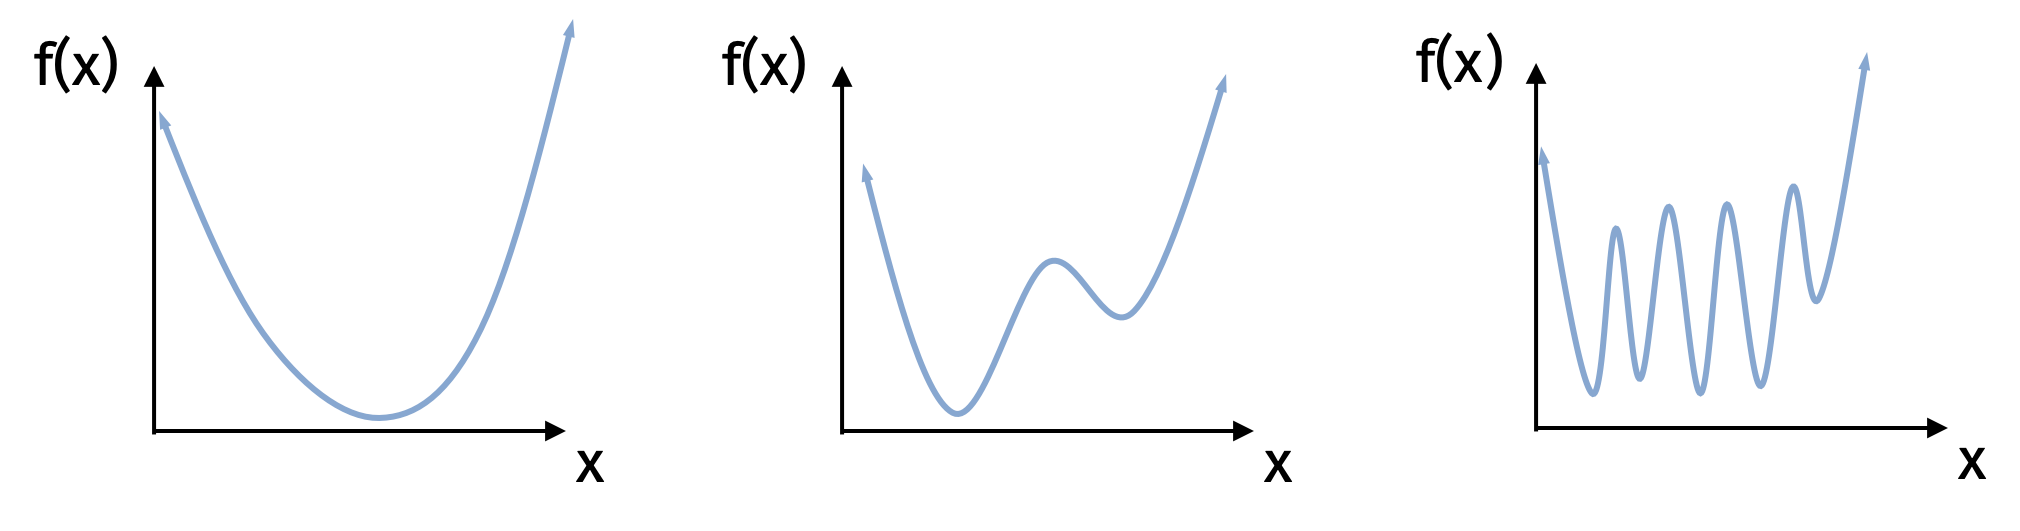
\includegraphics[width=\textwidth]{1d_functions.png}
	
	\textbf{Dimension $d = 2$:}
	
	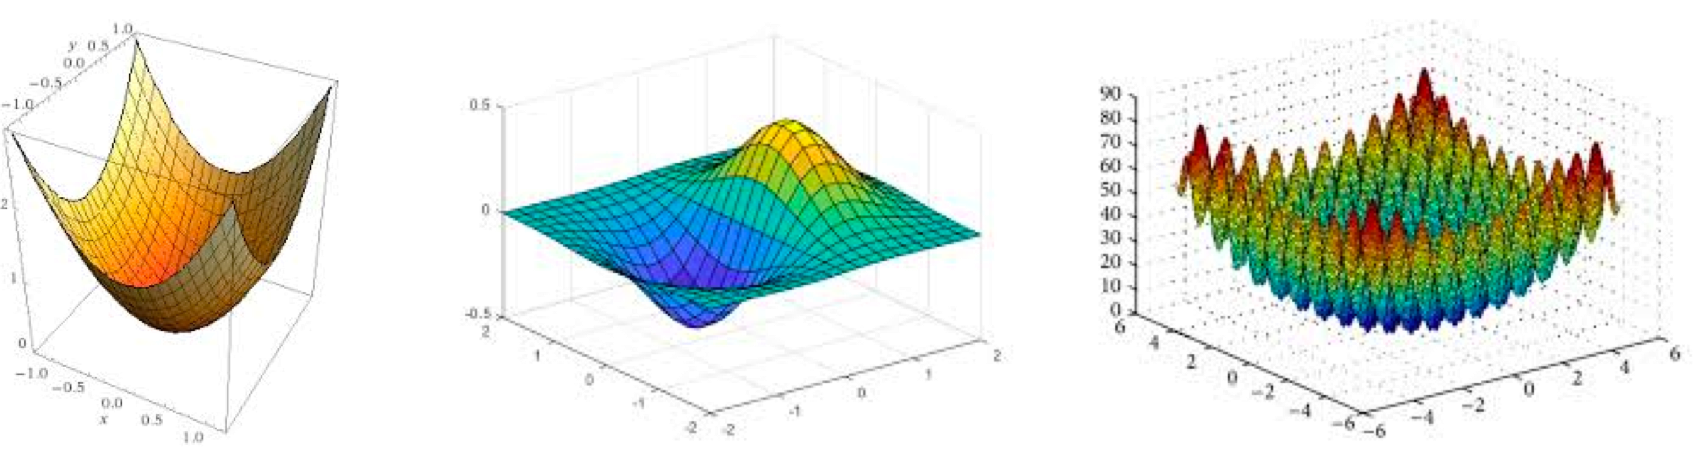
\includegraphics[width=\textwidth]{2dfunctions.png}
\end{frame}

\begin{frame}
	\frametitle{optimization in machine learning}
	\begin{center}
		\alert{\textbf{Continuouos optimization is the foundation of modern machine learning.}}
	\end{center}
	\textbf{Supervised learning:} Want to learn a model that maps \emph{inputs}
	\begin{itemize}
		\item numerical data vectors
		\item images, video
		\item a sequence of tokens/works
	\end{itemize} 
	
	to \emph{predictions}
	\begin{itemize}
		\item numerical value (probability stock price increases)
		\item label (does the image contain a car? what is the next token in the sequence?)
		\item decision (turn car left, rotate robotic arm)
	\end{itemize} 
\end{frame}

\begin{frame}
	\frametitle{machine learning model}
	\begin{center}
		Let $M_{\bv{x}}$ be a model with parameters $\bv{x} = \{x_1, \ldots, x_k\}$, which takes as input a data vector $\bv{a}$ and outputs a prediction.
	\end{center}
	
	\textbf{Example:}
	\begin{align*}
		M_{\bv{x}}(\bv{a}) = \sign(\bv{a}^T\bv{x})
	\end{align*}		
\end{frame}

\begin{frame}[t]
	\frametitle{machine learning model}
	\textbf{Example:}
	\begin{center}
		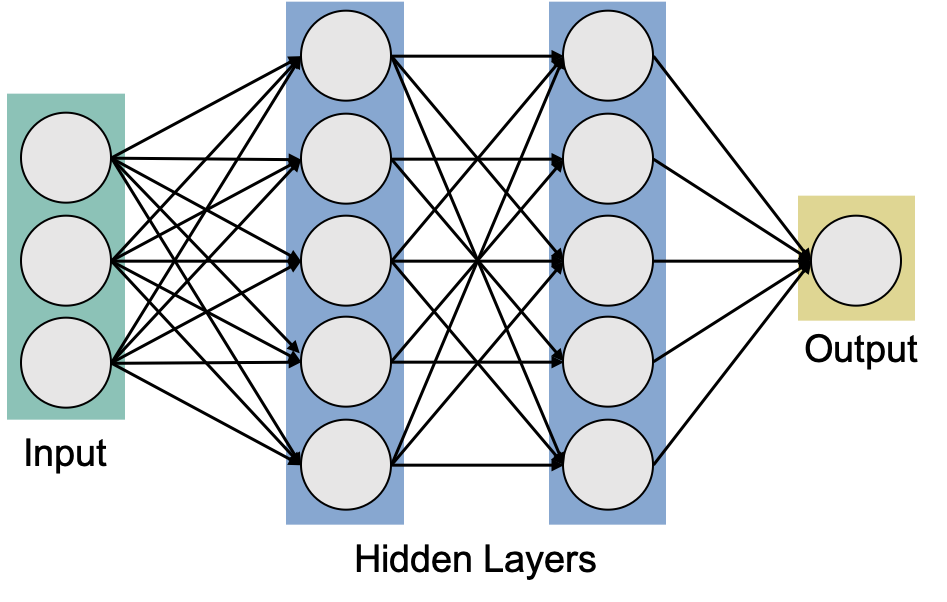
\includegraphics[width=.7\textwidth]{neuralNetwork.png}
	\end{center}	
	$\bv{x}\in \R^{\text{(\# of connections)}}$ is the parameter vector containing all the network weights. 	
\end{frame}

\begin{frame}
	\frametitle{supervised learning}
	Classic approach in \emph{supervised learning}: Find a model that works well on data that you already have the answer for (labels, values, classes, etc.).
	\begin{itemize}
		\item Model $M_{\bv{x}}$ parameterized by a vector of numbers $\bv{x}$.
		\item Dataset $\bv{a}^{(1)}, \ldots,  \bv{a}^{(n)}$ with outputs $y^{(1)}, \ldots, y^{(n)}$.
	\end{itemize}
	\begin{center}
		Want to find $\hat{\bv{x}}$ so that $M_{\hat{\bv{x}}}(\bv{a}^{(i)}) \approx y^{(i)}$ for $i \in 1,\ldots, n$.
		
		\alert{\textbf{How do we turn this into a function minimization problem?}}
	\end{center}
\end{frame}

\begin{frame}
	\frametitle{loss function}
	\textbf{Loss function $L\left(M_{\bv{x}}(\bv{a}), y\right)$:} Some measure of distance between prediction $M_{\bv{x}}(\bv{a})$ and target output $y$. Increases if they are further apart.
	\begin{itemize}
		\item Squared ($\ell_2$) loss: $|M_{{\bv{x}}}(\bv{a}) - y|^2$
		\item Absolute deviation ($\ell_1$) loss: $|M_{{\bv{x}}}(\bv{a}) - y|$
		\item Hinge loss: 1 - $y \cdot M_{{\bv{x}}}(\bv{a})$ 
		\item Cross-entropy loss (log loss). 
		%		$−o  \log(M_{{\bv{x}}}(\bv{y})+(1 - o)\log(1 - M_{{\bv{x}}}(\bv{y}))$
	\end{itemize}
\end{frame}

\begin{frame}
	\frametitle{empirical risk minimization}
	\textbf{Empirical risk minimization}: Given a training dataset $(\bv{a}^{(1)},y^{(1)}) \ldots,  (\bv{a}^{(n)},y^{(n)})$:
	\begin{align*}
		f(\bv{x}) = \sum_{i=1}^n L\left(M_{\bv{x}}(\bv{a}^{(i)}), y^{(i)}\right)
	\end{align*}
	\begin{center}
		Solve the optimization problem $\min_{\bv{x}} f(\bv{x})$.
	\end{center}
\end{frame}

\begin{frame}
	\frametitle{example: least squares regression}
	\begin{itemize}
		\item $M_{\bv{x}}(\bv{a}) = \bv{x}^T\bv{a}$. $\bv{x}$ contains the regression coefficients. 
		\item $L(z,y) = |z-y|^2$. 
		\item $f(\bv{x}) = \sum_{i=1}^n |\bv{x}^T\bv{a}^{(i)} - y^{(i)}|^2$
	\end{itemize}
	\begin{align*}
		f(\bv{x}) = \|\bv{A}\bv{x} - \bv{y}\|_2^2
	\end{align*}
	where $\bv{A}$ is a matrix with $\bv{a}^{(i)}$ as its $i^\text{th}$ row and $\bv{y}$ is a vector with $y^{(i)}$ as its $i^\text{th}$ entry. 
\end{frame}

\begin{frame}
	\frametitle{algorithms for continuous optimization}
	The choice of algorithm to minimize $f(\bv{x})$ will depend on:
	\begin{itemize}
		\item The form of $f(\bv{x})$ (is it linear, is it quadratic, does it have finite sum structure, etc.)
		\item If there are any additional constraints imposed on $\bv{x}$. E.g. $\|\bv{x}\|_2 \leq c$. 
	\end{itemize}
	\textbf{What are some example algorithms for continuous optimization?}
	
\end{frame}

\begin{frame}
	\frametitle{first topic: gradient descent + variants}
	\textbf{Gradient descent:} A greedy algorithm for minimizing functions of multiple variables that often works amazingly well. 
	\begin{center}
		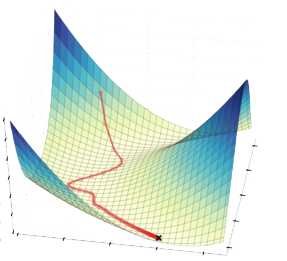
\includegraphics[width=.4\textwidth]{greedy_gradient.png}
		
		Runtime generally scales \emph{linearly} with the dimension of $\bv{x}$ (although this is a bit of an over-simplification).
	\end{center}
\end{frame}

\begin{frame}
	\frametitle{second topic: methods suitable for lower dimension }
	\begin{itemize}
		\item Cutting plane methods (e.g. center-of-gravity, ellipsoid)
		\item Interior point methods
	\end{itemize}
	Faster and more accurate in low-dimensions, slower in very high dimensions. Generally runtime scales \emph{polynomially} with the dimension of $\bv{x}$ (e.g., $O(d^3)$).
\end{frame}

\begin{frame}
	\frametitle{calculus review}
	For $i = 1, \ldots, d$, let $x_i$ be the $i^\text{th}$ entry of $\bv{x}$. Let $\bv{e}^{(i)}$ be the $i^\text{th}$ \emph{standard basis vector.}
	\vspace{2em}
	
	\textbf{Partial derivative:}
	\begin{align*}
		\frac{\partial f}{\partial x_i}(\bv{x}) = \lim_{t\rightarrow 0} \frac{f(\bv{x} + t\bv{e}^{(i)}) - f(\bv{x})}{t}
	\end{align*}
	\textbf{Directional derivative:}
	\begin{align*}
		D_\bv{v}f(\bv{x}) = \lim_{t\rightarrow 0} \frac{f(\bv{x} + t\bv{v}) - f(\bv{x})}{t}
	\end{align*}
\end{frame}

\begin{frame}
	\frametitle{calculus review}
	\textbf{Gradient}:
	\begin{align*}
		\nabla f(\bv{x}) = 
		\begin{bmatrix}
			\frac{\partial f}{\partial x_1}(\bv{x}) \\ \frac{\partial f}{\partial x_2}(\bv{x}) \\ \vdots \\ \frac{\partial f}{\partial x_d}(\bv{x}) 
		\end{bmatrix}
	\end{align*}
	\textbf{Directional derivative:}
	\begin{align*}
		D_\bv{v}f(\bv{x}) = \lim_{t\rightarrow 0} \frac{f(\bv{x} + t\bv{v}) - f(\bv{x})}{t} = \alert{\nabla f(\bv{x})^T \bv{v}.}
	\end{align*}
\end{frame}


\begin{frame}
	\frametitle{first order optimization}
	Given a function $f$ to minimize, assume we have:
	\begin{itemize}
		\item \textbf{Function oracle}: Evaluate $f(\bv{x})$ for any $\bv{x}$. 
		\item \textbf{Gradient oracle}: Evaluate $\nabla f(\bv{x})$ for any $\bv{x}$.
	\end{itemize}
	We view the implementation of these oracles as black-boxes, but they can often require a fair bit of computation. 
\end{frame}

\begin{frame}[t]
	\frametitle{example gradient evaluation}
	\textbf{Linear least-squares regression}:
	\begin{itemize}
		\item Given $\bv{a}^{(1)}, \ldots \bv{a}^{(n)} \in \R^d$, ${y}^{(1)}, \ldots {y}^{(n)} \in \R$.
		\item Want to minimize:
		\begin{align*}
			f(\bv{x}) = \sum_{i=1}^n \left(\bv{x}^T\bv{a}^{(i)} - {y}^{(i)}\right)^2 = \|\bv{A}\bv{x} - \bv{y}\|_2^2.
		\end{align*} 
	\end{itemize}
	\textbf{What is the time complexity to implement a function oracle for $f(\bv{x})$?}
\end{frame}

\begin{frame}[t]
	\frametitle{example gradient evaluation}
	\textbf{Linear least-squares regression}:
	\begin{itemize}
		\item Want to minimize:
		\begin{align*}
			f(\bv{x}) = \sum_{i=1}^n \left(\bv{x}^T\bv{a}^{(i)} - {y}^{(i)}\right)^2 = \|\bv{A}\bv{x} - \bv{y}\|_2^2.
		\end{align*} 
	\end{itemize}
	
	\begin{align*}
		\frac{\partial f}{\partial x_j} = \sum_{i=1}^n 2\left(\bv{x}^T\bv{a}^{(i)} - {y}^{(i)}\right)\cdot a^{(i)}_j = 2{\bs{\alpha}^{(j)}}^T(\bv{A}\bv{x} -\bv{y})
	\end{align*}
	where $\bs{\alpha}^{(j)}$ is the $j^\text{th}$ \emph{column} of $\bv{A}$. 
\end{frame}

\begin{frame}[t]
	\frametitle{example gradient evaluation}
	\textbf{Linear least-squares regression}:
	\begin{align*}
		\frac{\partial f}{\partial x_j} = \sum_{i=1}^n 2\left(\bv{x}^T\bv{a}^{(i)} - {y}^{(i)}\right)\cdot a^{(i)}_j = 2{\bs{\alpha}^{(j)}}^T(\bv{A}\bv{x} -\bv{y})
	\end{align*}
	where $\bs{\alpha}^{(j)}$ is the $j^\text{th}$ \emph{column} of $\bv{A}$. 
	\begin{align*}
		\nabla f(\bv{x}) = 2\bv{A}^T\left(\bv{A}\bv{x} - \bv{y}\right)
	\end{align*}
	\textbf{What is the time complexity of a gradient oracle for $\nabla f(\bv{x})$?}
\end{frame}

\begin{frame}
	\frametitle{descent methods}
	\textbf{Greedy approach:} Given a starting point $\bv{x}$, make a small adjustment that decreases $f(\bv{x})$. In particular, $\bv{x} \leftarrow \bv{x} + \eta\bv{v}$.
	
	\begin{center}
		\alert{What property do I want in $\bv{v}$?}
	\end{center}
	
	
	\textbf{Leading question:} When $\eta$ is small, what's an approximation for $f(\bv{x} + \eta\bv{v}) - f(\bv{x})$?
	\begin{align*}
		f(\bv{x} + \eta\bv{v}) - f(\bv{x}) \approx \hspace{6em}
	\end{align*}
	
	
\end{frame}

\begin{frame}[t]
	\frametitle{directional derivatives}
	
	\begin{align*}
		D_\bv{v}f(\bv{x}) = \lim_{t\rightarrow 0} \frac{f(\bv{x} + t\bv{v}) - f(\bv{x})}{t} = \nabla f(\bv{x})^T \bv{v}.
	\end{align*}	
	So:
	\begin{align*}
		f(\bv{x} + \eta\bv{v}) - f(\bv{x}) \approx \eta \cdot \nabla f(\bv{x})^T \bv{v}.
	\end{align*}
	
	\textbf{How should we choose $\bv{v}$ so that $f(\bv{x} + \eta\bv{v}) < f(\bv{x})$?} 
	
\end{frame}

\begin{frame}
	\frametitle{gradient descent}
	\textbf{Prototype algorithm:}
	\begin{itemize}
		\item Choose starting point $\bv{x}^{(0)}$.
		\item For $i = 0,\ldots, T$:
		\begin{itemize}
			\item $\bv{x}^{(i+1)} = \bv{x}^{(i)} - \eta \nabla f(\bv{x}^{(i)})$
		\end{itemize}
		\item Return $\bv{x}^{(T)}$.
	\end{itemize}
	
	$\eta$ is a step-size parameter, which is often adapted on the go. For now, assume it is fixed ahead of time.
\end{frame}

\begin{frame}[t]
	\frametitle{gradient descent intuition}
	\textbf{1 dimensional example:}
\end{frame}

\begin{frame}[t]
	\frametitle{gradient descent intuition}
	\textbf{2 dimensional example:}
	\begin{center}
		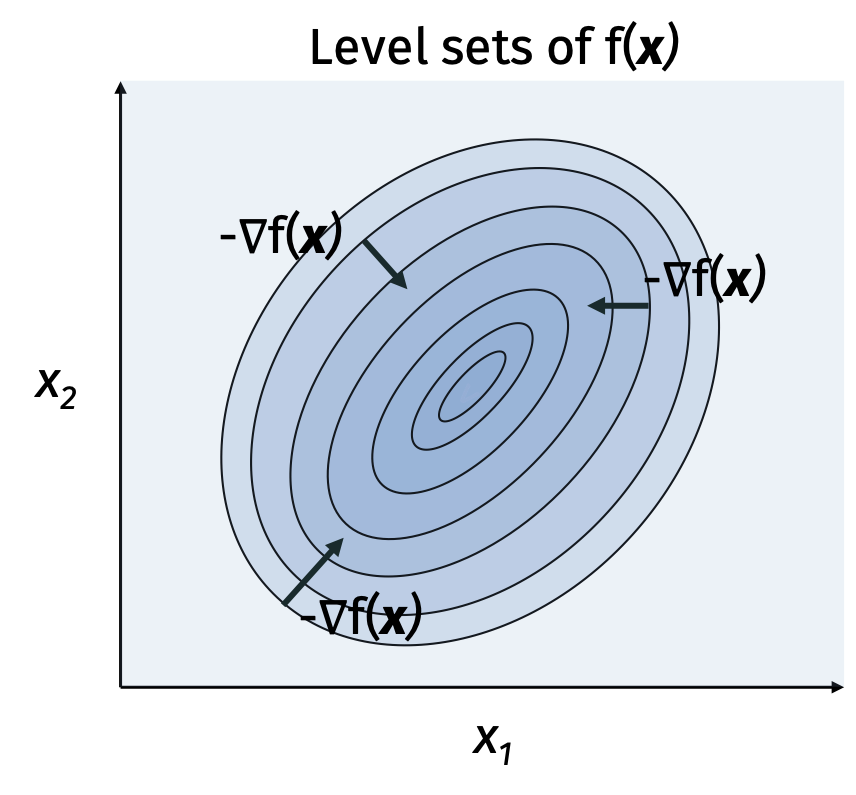
\includegraphics[width=.7\textwidth]{2d_example.png}
	\end{center}
\end{frame}

\begin{frame}[t]
	\frametitle{key results}
	\textbf{For a convex function $f(\bv{x})$:}
	For sufficiently small $\eta$ and a sufficiently large number of iterations $T$, gradient descent will converge to a \alert{\textbf{near global minimum}}:
	\begin{align*}
		f(\bv{x}^{(T)}) \leq  f(\bv{x}^{*}) + \epsilon.  
	\end{align*}
	Examples: least squares regression, logistic regression, kernel regression, SVMs.
	
	\textbf{For a non-convex function $f(\bv{x})$:}
	For sufficiently small $\eta$ and  a sufficiently large number of iterations $T$, gradient descent will converge to a \alert{\textbf{near stationary point}}:
	\begin{align*}
		\|\nabla f(\bv{x}^{(T)})\|_2 \leq  \epsilon.  
	\end{align*}
	Examples: neural networks, matrix completion problems, mixture models. 	
\end{frame}

\begin{frame}[t]
	\frametitle{convex vs. non-convex}
	\begin{center}
		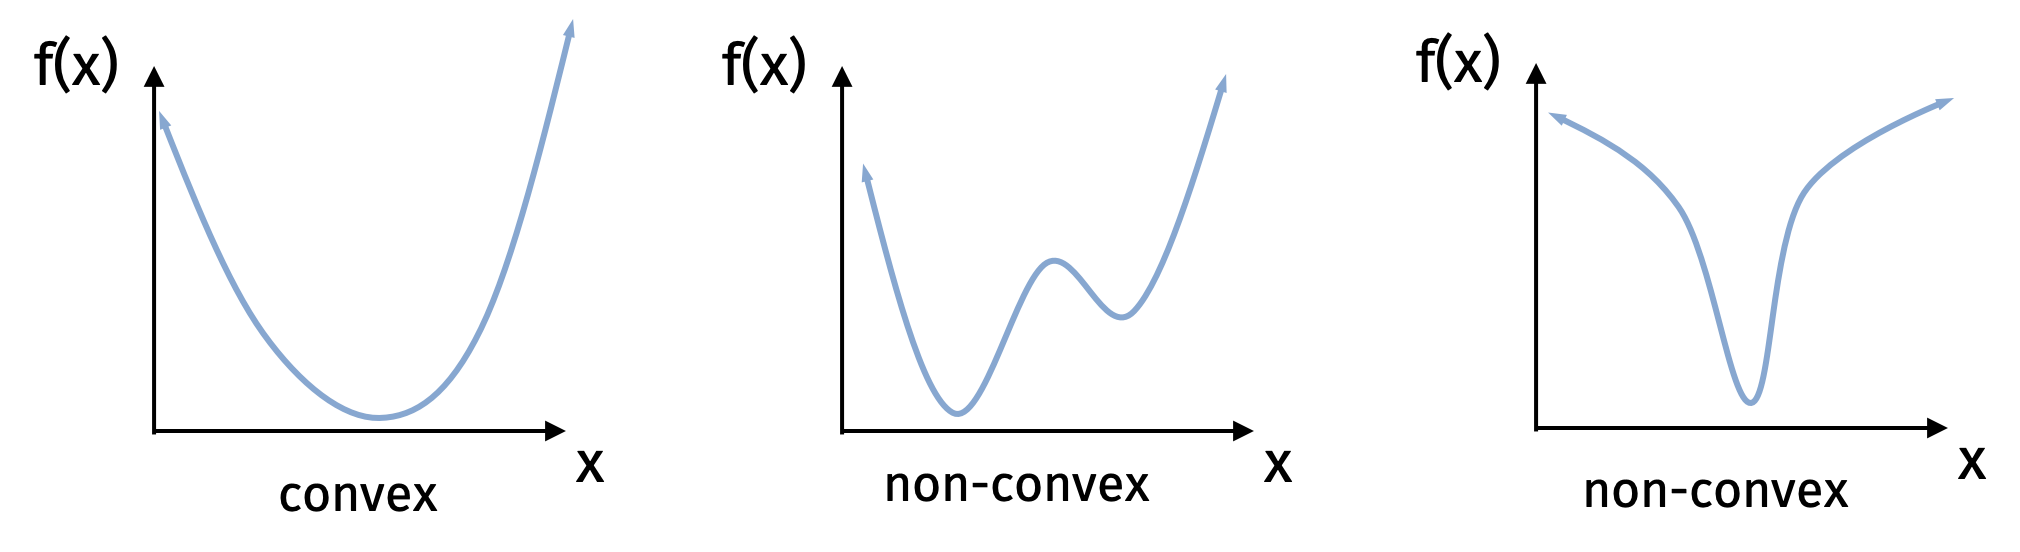
\includegraphics[width=\textwidth]{nonconvex_converge.png}
	\end{center}
	One issue with non-convex functions is that they can have \alert{\textbf{local minima}}. Even when they don't, convergence analysis requires different assumptions than convex functions. 	
\end{frame}

\begin{frame}[t]
	\frametitle{approach for this unit}
	We care about \emph{how fast} gradient descent and related methods converge, not just that they do converge. 
	\begin{itemize}
		\item Bounding iteration complexity requires placing some assumptions on $f(\bv{x})$. 
		\item Stronger assumptions lead to better bounds on the convergence. 
	\end{itemize}
	Understanding these assumptions can help us design faster variants of gradient descent (there are many!). 
	
	\begin{center}
		Today, we will start with \textbf{convex} functions. 
	\end{center}
\end{frame}

\begin{frame}[t]
	\frametitle{convexity}
	\begin{definition}[Convex]
		A function $f$ is convex iff for any $\bv{x}, \bv{y},\lambda \in [0,1]$:
		\begin{align*}
		(1-\lambda)\cdot f(\bv{x}) + \lambda \cdot f(\bv{y}) \geq f\left((1-\lambda)\cdot\bv{x} + \lambda \cdot\bv{y}\right)
		\end{align*}
	\end{definition}
\vspace{-.5em}
\begin{center}
	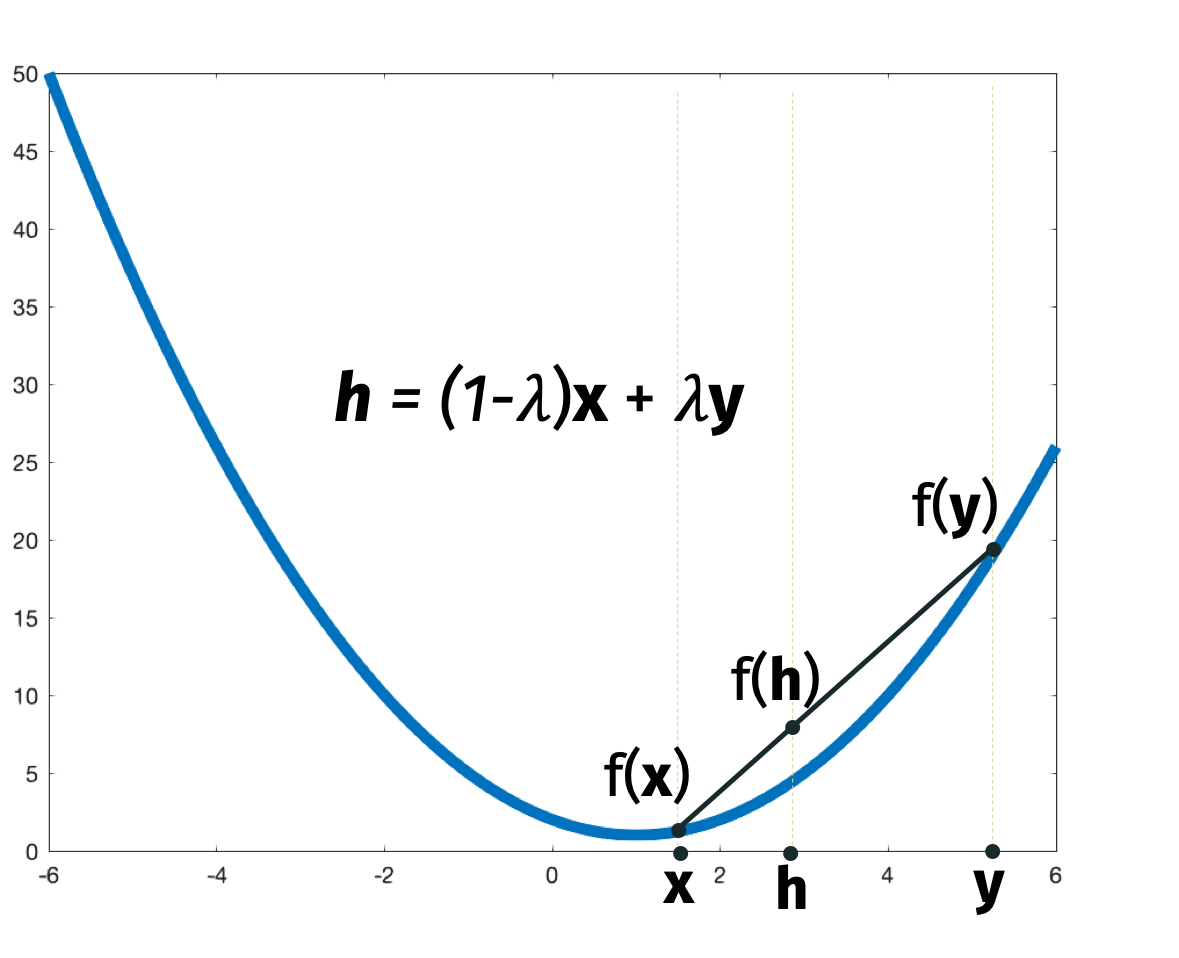
\includegraphics[width=.6\textwidth]{convex1.png}
\end{center}
\end{frame}


\begin{frame}[t]
	\frametitle{gradient descent}
	\small
		\begin{definition}[Convex]
		A function $f$ is convex if and only if for any $\bv{x}, \bv{y}$:
		\begin{align*}
			f(\bv{x} + \bv{z}) \geq f(\bv{x}) + \nabla f(\bv{x})^T\bv{z}
		\end{align*}
	\vspace{-1em}
	Equivalently:
	\vspace{-.5em}
		\begin{align*}
			f(\bv{x}) - f(\bv{y}) \leq \nabla f(\bv{x})^T (\bv{x} - \bv{y})
		\end{align*}
	\vspace{-1em}
	\end{definition}

	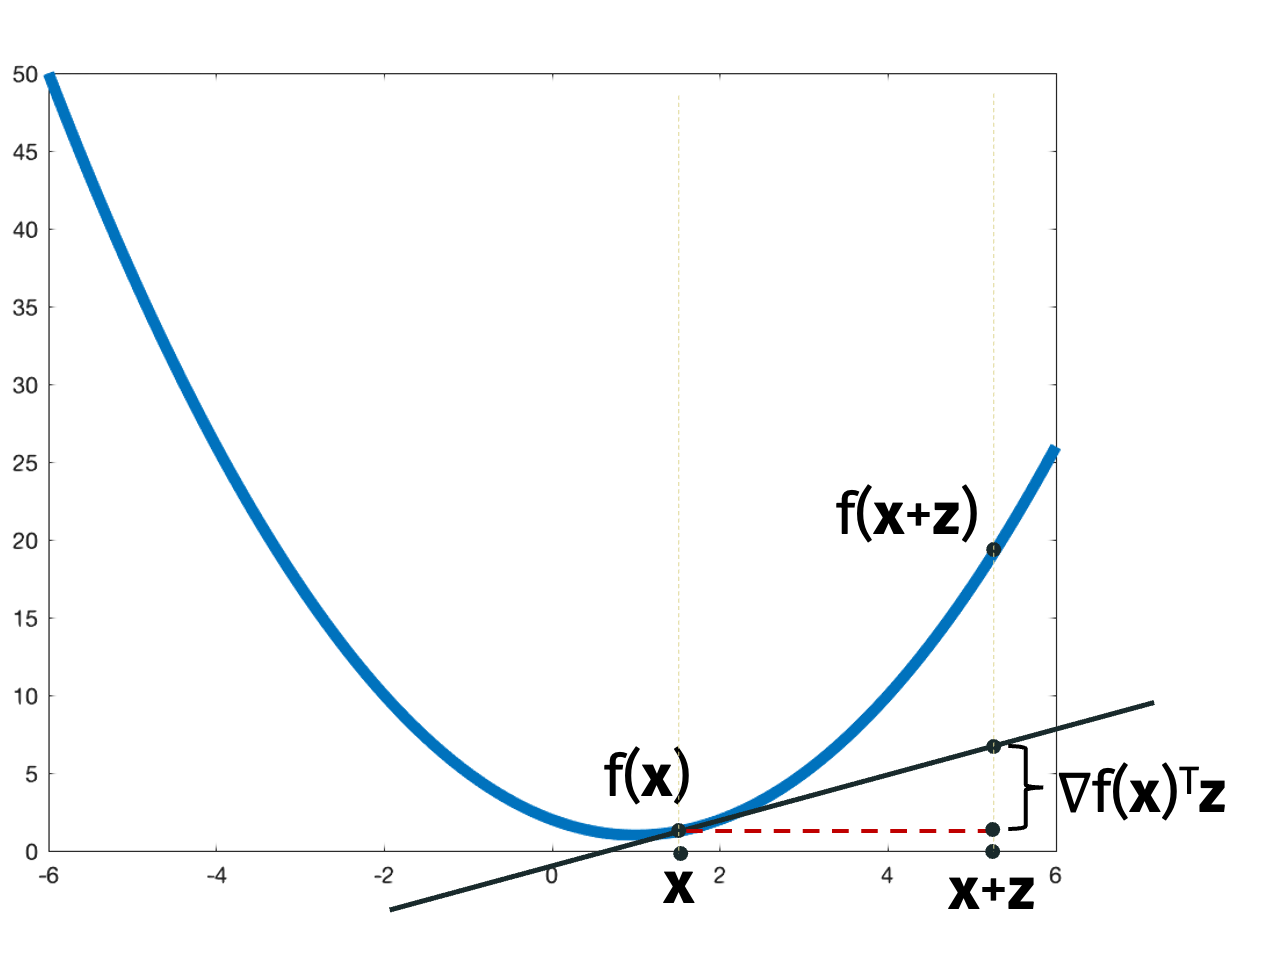
\includegraphics[width=.5\textwidth]{convex2.png}

\end{frame}

\begin{frame}
	\frametitle{definitions of convexity}
	It is easy but not obvious how to prove the equivalence between these definitions. A short proof can be found in Karthik Sridharan's lecture notes here:
	\begin{center}
		\color{blue}
		\href{http://www.cs.cornell.edu/courses/cs6783/2018fa/lec16-supplement.pdf}{http://www.cs.cornell.edu/courses/cs6783/2018fa/lec16-supplement.pdf}
	\end{center}
	
\end{frame}

\begin{frame}[t]
	\frametitle{gradient descent analysis}
	\textbf{Assume:}
	\begin{itemize}
		\item $f$ is convex.
		\item Lipschitz function: for all $\bv{x}$, $\|\nabla f(\bv{x})\|_2 \leq \alert{G}$.
		\item Starting radius: $\|\bv{x}^{*} - \bv{x}^{(0)}\|_2 \leq \alert{R}$.
	\end{itemize}
	
	\textbf{Gradient descent:}
	\begin{itemize}
		\item Choose number of steps $T$.
		\item Starting point $\bv{x}^{(0)}$. E.g.  $\bv{x}^{(0)} = \vec{0}$.
		\item $\eta = \frac{R}{G\sqrt{T}}$
		\item For $i = 0,\ldots, T$:
		\begin{itemize}
			\item $\bv{x}^{(i+1)} = \bv{x}^{(i)} - \eta \nabla f(\bv{x}^{(i)})$
		\end{itemize}
		\item Return $\hat{\bv{x}} = \argmin_{\bv{x}^{(i)}} f(\bv{x}^{(i)})$.
%		\item Alternatively, return $\hat{\bv{x}} = \frac{1}{T}\sum_{i=1}^T \bv{x}^{(i)}$.
	\end{itemize}
\end{frame}

\begin{frame}[t]
	\frametitle{gradient descent analysis}
	\begin{claim}[GD Convergence Bound]
		If we run GD for $T \geq \frac{R^2G^2}{\epsilon^2}$ iterations then $f(\hat{\bv{x}}) \leq f(\bv{x}^*) + \epsilon$.
	\end{claim}


	\vspace{12em}
	Proof is made tricky by the fact that $f(\bv{x}^{(i)})$ does not improve monotonically. We can ``overshoot" the minimum. 
\end{frame}

\begin{frame}[t]
	\frametitle{gradient descent analysis}
	\begin{claim}[GD Convergence Bound]
		If we run GD for $T \geq \frac{R^2G^2}{\epsilon^2}$ iterations with step-size $\eta = \frac{R}{G\sqrt{T}}$, then $f(\hat{\bv{x}}) \leq f(\bv{x}^*) + \epsilon$.
	\end{claim}

	Proof is made tricky by the fact that $f(\bv{x}^{(i)})$ does not improve monotonically. We can ``overshoot" the minimum. 
	
	We will prove that the \emph{average} solution value is low after $T = \frac{R^2G^2}{\epsilon^2}$ iterations. I.e. that:
	\begin{align*}
		\frac{1}{T}\sum_{i=0}^{T-1}\left[f(\bv{x}^{(i)}) - f(\bv{x}^*)\right]  \leq \epsilon \hspace{15em}
	\end{align*}
Of course the best solution found, $\hat{\bv{x}}$ is only better than the average.
\end{frame}

\begin{frame}[t]
	\frametitle{gradient descent analysis}
	\small
	\begin{claim}[GD Convergence Bound]
		If we run GD for $T \geq \frac{R^2G^2}{\epsilon^2}$ iterations with step-size $\eta = \frac{R}{G\sqrt{T}}$, then $f(\hat{\bv{x}}) \leq f(\bv{x}^*) + \epsilon$.
	\end{claim}
	\textbf{Claim 1:} For all $i = 0, \ldots, T$, 
	\begin{align*}
		f(\bv{x}^{(i)}) - f(\bv{x}^*) \leq \frac{\|\bs{x}^{(i)} - \bs{x}^*\|_2^2 - \|\bs{x}^{(i+1)} -\bs{x}^*\|_2^2}{2\eta} + \frac{\eta G^2}{2}
	\end{align*}
	
	\textbf{Claim 1(a):} For all $i = 0, \ldots, T$, 
	\begin{align*}
		\nabla f(\bv{x}^{(i)})^T(\bs{x}^{(i)} - \bs{x}^{*})  \leq \frac{\|\bs{x}^{(i)} - \bs{x}^*\|_2^2 - \|\bs{x}^{(i+1)} -\bs{x}^*\|_2^2}{2\eta} + \frac{\eta G^2}{2}
	\end{align*}
	
	Claim 1 follows from Claim 1(a) by definition of convexity.
\end{frame}

\begin{frame}[t]
	\frametitle{gradient descent analysis}
	\small
	\begin{claim}[GD Convergence Bound]
		If we run GD for $T \geq \frac{R^2G^2}{\epsilon^2}$ iterations with step size $\eta = \frac{R}{G\sqrt{T}}$, then $f(\hat{\bv{x}}) \leq f(\bv{x}^*) + \epsilon$.
	\end{claim}
	\textbf{Claim 1(a):} For all $i = 0, \ldots, T$, 
	\begin{align*}
		 \frac{\|\bv{x}^{(i)} - \bv{x}^*\|_2^2 - \|\bv{x}^{(i+1)} -\bv{x}^*\|_2^2}{2\eta} + \frac{\eta G^2}{2} \geq \nabla f(\bv{x}^{(i)})^T(\bv{x}^{(i)} - \bv{x}^{*})
	\end{align*}
\end{frame}

%\begin{frame}[t]
%	\frametitle{gradient descent analysis}
%	\small
%	\begin{claim}[GD Convergence Bound]
%		If $T \geq \frac{R^2G^2}{\epsilon^2}$ and $\eta = \frac{R}{G\sqrt{T}}$, then $f(\hat{\bv{x}}) \leq f(\bv{x}^*) + \epsilon$.
%	\end{claim}
%	\textbf{Claim 1:} For all $i = 0, \ldots, T$, 
%	\begin{align*}
%		f(\bv{x}^{(i)}) - f(\bv{x}^*) \leq \frac{\|\bv{x}^{(i)} - \bv{x}^*\|_2^2 - \|\bv{x}^{(i+1)} - \bv{x}^*\|_2^2}{2\eta} + \frac{\eta G^2}{2}
%	\end{align*}
%	\textbf{Telescoping sum:}
%	\begin{align*}
%		\sum_{i=0}^{T-1}\left[f(\bv{x}^{(i)}) - f(\bv{x}^*)\right] &\leq \frac{\|\bv{x}^{(0)} - \bv{x}^*\|_2^2 - \|\bv{x}^{(T)} - \bv{x}^*\|_2^2}{2\eta} + \frac{T\eta G^2}{2}\\
%		\frac{1}{T}\sum_{i=0}^{T-1}\left[f(\bv{x}^{(i)}) - f(\bv{x}^*)\right] &\leq \frac{R^2}{2T\eta} + \frac{\eta G^2}{2}
%	\end{align*}
%\end{frame}
%
%\begin{frame}[t]
%	\frametitle{gradient descent analysis}
%	\small
%	\textbf{Telescoping sum:}
%	\begin{align*}
%		\sum_{i=0}^{T-1}\left[f(\bv{x}^{(i)}) - f(\bv{x}^*)\right] &\leq \frac{\|\bv{x}^{(0)} - \bv{x}^*\|_2^2 - \|\bv{x}^{(T)} - \bv{x}^*\|_2^2}{2\eta} + \frac{T\eta G^2}{2}\\
%		\frac{1}{T}\sum_{i=0}^{T-1}\left[f(\bv{x}^{(i)}) - f(\bv{x}^*)\right] &\leq \frac{R^2}{2T\eta} + \frac{\eta G^2}{2}
%	\end{align*}
%\end{frame}
%
%\begin{frame}[t]
%	\frametitle{gradient descent analysis}
%	\begin{claim}[GD Convergence Bound]
%		If $T \geq \frac{R^2G^2}{\epsilon^2}$ and $\eta = \frac{R}{G\sqrt{T}}$, then $f(\hat{\bv{x}}) \leq f(\bv{x}^*) + \epsilon$.
%	\end{claim}
%	\textbf{Final step:}
%	\begin{align*}
%		\frac{1}{T}\sum_{i=0}^{T-1}\left[f(\bv{x}^{(i)}) - f(\bv{x}^*)\right] &\leq \epsilon \\ 
%		\left[\frac{1}{T}\sum_{i=0}^{T-1}f(\bv{x}^{(i)})\right] - f(\bv{x}^*) &\leq \epsilon 
%	\end{align*}
%	We always have that $\min_i f(\bv{x}^{(i)}) \leq \frac{1}{T}\sum_{i=0}^{T-1}f(\bv{x}^{(i)})$, so this is what we return:
%	\begin{align*}
%		L(\hat{\bv{x}}) = \min_{i\in 1,\ldots, T} f(\bv{x}^{(i)}) \leq f(\bv{x}^*) + \epsilon. 
%	\end{align*}
%\end{frame}

%\begin{frame}[t]
%	\frametitle{gradient descent analysis}
%	\begin{claim}[GD Convergence Bound]
%		If $T \geq \frac{R^2G^2}{\epsilon^2}$ and $\eta = \frac{R}{G\sqrt{T}}$, then $f(\hat{\bv{x}}) \leq f(\bv{x}^*) + \epsilon$.
%	\end{claim}
%\textbf{Claim 1:} For all $i = 0, \ldots, T$, 
%\begin{align*}
%	f(\bv{x}^{(i)}) - f(\bv{x}^*) \leq \frac{\|\bv{x}^{(i)} - \bv{x}^*\|_2^2 - \|\bv{x}^{(i+1)} - \bv{x}^*\|_2^2}{2\eta} + \frac{\eta G^2}{2}
%\end{align*}
%
%\end{frame}

\begin{frame}[t]
	\frametitle{gradient descent analysis}
	\footnotesize
	\begin{claim}[GD Convergence Bound]
		If $T \geq \frac{R^2G^2}{\epsilon^2}$ and $\eta = \frac{R}{G\sqrt{T}}$, then $f(\bv{\hat{x}}) \leq f(\bv{x}^*) + \epsilon$.
	\end{claim}
	\textbf{Claim 1:} For all $i = 0, \ldots, T$, 
	\begin{align*}
		f(\bv{x}^{(i)}) - f(\bv{x}^*) \leq \frac{\|\bv{x}^{(i)} - \bv{x}^*\|_2^2 - \|\bv{x}^{(i+1)} - \bv{x}^*\|_2^2}{2\eta} + \frac{\eta G^2}{2}
	\end{align*}
	\textbf{Telescoping sum:}
	\begin{align*}
		\sum_{i=0}^{T-1}\left[f(\bv{x}^{(i)}) - f(\bv{x}^*)\right] &\leq \frac{\|\bv{x}^{(0)} - \bv{x}^*\|_2^2 - \|\bv{x}^{(1)} - \bv{x}^*\|_2^2}{2\eta} + \frac{\eta G^2}{2}\\
		&+ \frac{\|\bv{x}^{(1)} - \bv{x}^*\|_2^2 - \|\bv{x}^{(2)} - \bv{x}^*\|_2^2}{2\eta} + \frac{\eta G^2}{2}\\
		&+ \frac{\|\bv{x}^{(2)} - \bv{x}^*\|_2^2 - \|\bv{x}^{(3)} - \bv{x}^*\|_2^2}{2\eta} + \frac{\eta G^2}{2}\\
		&\vdots\\
		&+ \frac{\|\bv{x}^{(T-1)} - \bv{x}^*\|_2^2 - \|\bv{x}^{(T)} - \bv{x}^*\|_2^2}{2\eta} + \frac{\eta G^2}{2}
	\end{align*}
	
	\begin{align*}
		\sum_{i=0}^{T-1}\left[f(\bv{x}^{(i)}) - f(\bv{x}^*)\right] &\leq \frac{\|\bv{x}^{(0)} - \bv{x}^*\|_2^2 - \|\bv{x}^{(T)} - \bv{x}^*\|_2^2}{2\eta} + \frac{T\eta G^2}{2}\\
		\frac{1}{T}\sum_{i=0}^{T-1}\left[f(\bv{x}^{(i)}) - f(\bv{x}^*)\right] &\leq \frac{R^2}{2T\eta} + \frac{\eta G^2}{2}
	\end{align*}
\end{frame}

\begin{frame}[t]
	\frametitle{gradient descent analysis}
	\small
	\begin{claim}[GD Convergence Bound]
	If $T \geq \frac{R^2G^2}{\epsilon^2}$ and $\eta = \frac{R}{G\sqrt{T}}$, then $f(\bv{\hat{x}}) \leq f(\bv{x}^*) + \epsilon$.
	\end{claim}
\textbf{Telescoping sum:}
\begin{align*}
	\sum_{i=0}^{T-1}\left[f(\bv{x}^{(i)}) - f(\bv{x}^*)\right] &\leq \frac{\|\bv{x}^{(0)} - \bv{x}^*\|_2^2 - \|\bv{x}^{(T)} - \bv{x}^*\|_2^2}{2\eta} + \frac{T\eta G^2}{2}\\
	\frac{1}{T}\sum_{i=0}^{T-1}\left[f(\bv{x}^{(i)}) - f(\bv{x}^*)\right] &\leq \frac{R^2}{2T\eta} + \frac{\eta G^2}{2}
\end{align*}
\end{frame}
\begin{frame}[t]
	\frametitle{gradient descent analysis}
	\begin{claim}[GD Convergence Bound]
		If $T \geq \frac{R^2G^2}{\epsilon^2}$ and $\eta = \frac{R}{G\sqrt{T}}$, then $f(\hat{\bv{x}}) \leq f(\bv{x}^*) + \epsilon$.
	\end{claim}
	\textbf{Final step:}
	\begin{align*}
		\frac{1}{T}\sum_{i=0}^{T-1}\left[f(\bv{x}^{(i)}) - f(\bv{x}^*)\right] &\leq \epsilon \\ 
		\left[\frac{1}{T}\sum_{i=0}^{T-1}f(\bv{x}^{(i)})\right] - f(\bv{x}^*) &\leq \epsilon 
	\end{align*}
We always have that $f(\hat{\bv{x}}) = \min_i f(\bv{x}^{(i)}) \leq \frac{1}{T}\sum_{i=0}^{T-1}f(\bv{x}^{(i)})$, which gives the final bound:
\begin{align*}
	f(\hat{\bv{x}}) \leq f(\bv{x}^*) + \epsilon. 
\end{align*}
\end{frame}

\begin{frame}[t]
	\frametitle{constrained convex optimization}
	\textbf{Typical goal}: Solve a \emph{convex minimization problem} with additional \emph{convex constraints}.  
	\begin{align*}
		\min_{\bv{x}\in \mathcal{S}} f(\bv{x})
	\end{align*}
where $\mathcal{S}$ is a \textbf{\alert{convex set}}. 
\begin{center}
	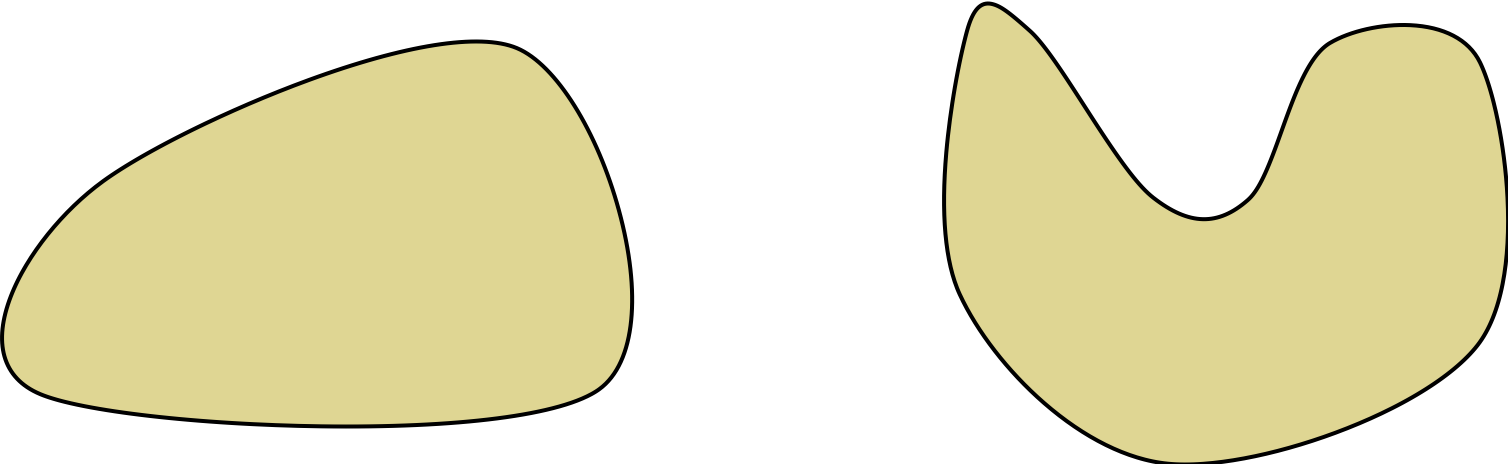
\includegraphics[width=.7\textwidth]{sets.png}
	
	Which of these is convex?
\end{center}
\end{frame}

\begin{frame}[t]
	\frametitle{constrained convex optimization}
	\begin{center}
		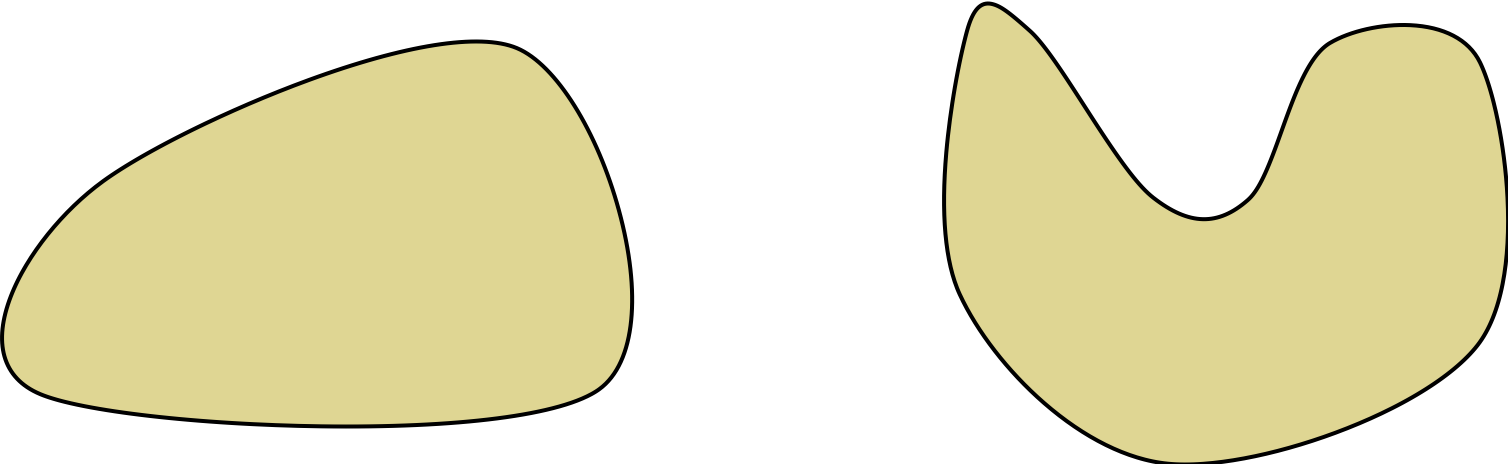
\includegraphics[width=.7\textwidth]{sets.png}
	\end{center}

	\begin{definition}[Convex set]
		A set $\mathcal{S}$ is convex if for any $\bv{x}, \bv{y} \in \mathcal{S}, \lambda \in [0,1]$:
		\begin{align*}
			(1-\lambda)\bv{x} + \lambda\bv{y} \in \mathcal{S}.
		\end{align*}
	\end{definition}
\end{frame}

\begin{frame}[t]
	\frametitle{constrained convex optimization}
	\textbf{Examples:}
	\begin{itemize}
		\item \textbf{Norm constraint:} minimize $\|\bv{A}\bv{x} - \bv{b}\|_2$ subject to $\|\bv{x}\|_2 \leq \lambda$. Used e.g. for regularization, finding a sparse solution, etc.
		\item \textbf{Positivity constraint:} minimize $f(\bv{x})$ subject to $\bv{x} \geq 0$. 
		% Used e.g. in finding an optimal allocation for a portfolio into different assets. 
		\item \textbf{Linear constraint:} minimize $\bv{c}^T\bv{x}$ subject to $\bv{A}\bv{x} \leq \bv{b}$. Linear program used in training support vector machines, industrial optimization, subroutine in integer programming, etc.
	\end{itemize}
\end{frame}

\begin{frame}[t]
	\frametitle{problem with gradient descent}
	\textbf{Gradient descent:}
	\begin{itemize}
		\item For $i = 0,\ldots, T$:
		\begin{itemize}
			\item $\bv{x}^{(i+1)} = \bv{x}^{(i)} - \eta \nabla f(\bv{x}^{(i)})$
		\end{itemize}
		\item Return $\hat{\bv{x}} = \argmin_{i} f(\bv{x}^{(i)})$.
	\end{itemize}
	
	\begin{center}
		\alert{
		Even if we start with $\bv{x}^{(0)} \in \mathcal{S}$, there is no guarantee that $ \bv{x}^{(0)} - \eta \nabla f(\bv{x}^{(0)})$ will remain in our set.}
	\end{center}

	\textbf{Extremely simple modification:} Force $\bv{x}^{(i)}$ to be in $\mathcal{S}$ by \textbf{\alert{projecting}} onto the set.
\end{frame}

\begin{frame}
	\frametitle{constrained first order optimization}
	Given a function $f$ to minimize and a convex constraint set $\mathcal{S}$, assume we have:
	\begin{itemize}
		\item \textbf{Function oracle}: Evaluate $f(\bv{x})$ for any $\bv{x}$. 
		\item \textbf{Gradient oracle}: Evaluate $\nabla f(\bv{x})$ for any $\bv{x}$.
		\item \textbf{\alert{Projection oracle}}: Evaluate $P_{\mathcal{S}}(\bv{x})$ for any $\bv{x}$.
	\end{itemize}
\begin{align*}
	P_{\mathcal{S}}(\bv{x}) = \argmin_{\bv{y}\in \mathcal{S}} \|\bv{x} - \bv{y}\|_2
\end{align*}
\end{frame}

\begin{frame}
	\frametitle{projection oracles}
	\begin{itemize}
		\item How would you implement $P_\mathcal{S}$ for $\mathcal{S} = \{\bv{y}:\|\bv{y}\|_2\leq 1\}.$
		\item How would you implement $P_\mathcal{S}$ for $\mathcal{S} = \{\bv{y}:\bv{y} = \bv{Q}\bv{z}\}.$
	\end{itemize}
\begin{center}
	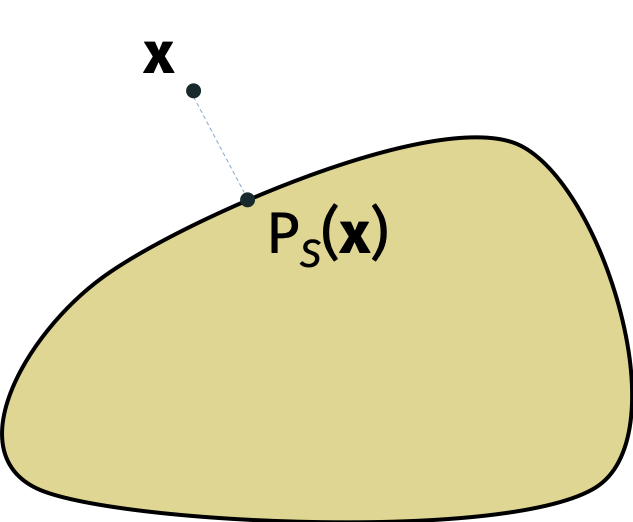
\includegraphics[width=.5\textwidth]{projection_image.png}
\end{center}
\end{frame}

\begin{frame}[t]
	\frametitle{projected gradient descent}
	Given function $f(\bv{x})$ and set $\mathcal{S}$, such that $\|\nabla f(\bv{x})\|_2 \leq G$ for all $\bv{x}\in \mathcal{S}$ and starting point $\bv{x}^{(0)}$ with $\|\bv{x}^{(0)} - \bv{x}^*\|_2 \leq R$.  
	
	\textbf{Projected gradient descent:}
	\begin{itemize}
		\item Select starting point $\bv{x}^{(0)}$, $\eta = \frac{R}{G\sqrt{T}}$. 
		\item For $i = 0,\ldots, T$:
		\begin{itemize}
			\item $\bv{z} = \bv{x}^{(i)} - \eta \nabla f(\bv{x}^{(i)})$
			\item $\bv{x}^{(i+1)} = P_\mathcal{S}(\bv{z})$
		\end{itemize}
		\item Return $\hat{\bv{x}} = \argmin_{i} f(\bv{x}^{(i)})$.
	\end{itemize}
\begin{claim}[PGD Convergence Bound]
	If $f, \mathcal{S}$ are convex and $T \geq \frac{R^2G^2}{\epsilon^2}$, then $f(\hat{\bv{x}}) \leq f(\bv{x}^*) + \epsilon$.
\end{claim}
\end{frame}

\begin{frame}[t]
	\frametitle{projected gradient descent analysis}
	Analysis is almost identical to standard gradient descent! We just need one additional claim:
	
	\begin{claim}[Contraction Property of Convex Projection]
		If $\mathcal{S}$ is convex, then for \emph{any} $\bv{y} \in \mathcal{S}$,
		\begin{align*}
			\|\bv{y} - P_\mathcal{S}(\bv{x})\|_2 \leq \|\bv{y} - \bv{x}\|_2.
		\end{align*}
	\end{claim}
\vspace{-1em}
\begin{center}
	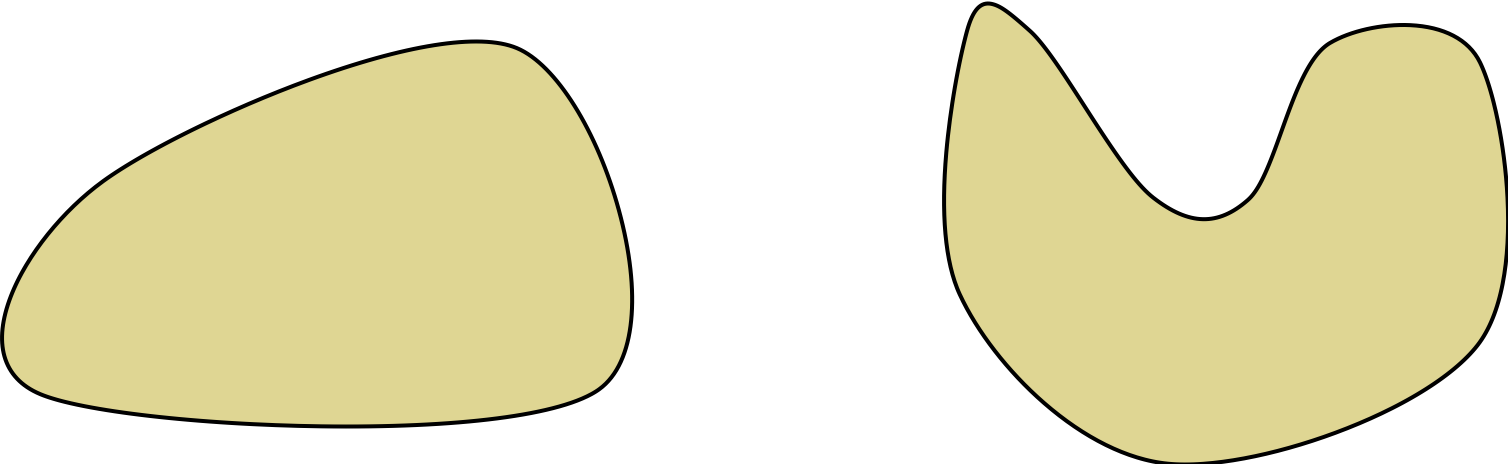
\includegraphics[width=.8\textwidth]{sets.png}
\end{center}	
\end{frame}

\begin{frame}[t]
	\frametitle{gradient descent analysis}
	\small
\begin{claim}[PGD Convergence Bound]
	If $f, \mathcal{S}$ are convex and $T \geq \frac{R^2G^2}{\epsilon^2}$, then $f(\hat{\bv{x}}) \leq f(\bv{x}^*) + \epsilon$.
\end{claim}
	\textbf{Claim 1:} For all $i = 0, \ldots, T$, let $\bv{z}^{(i)} = \bv{x}^{(i)} - \eta \nabla f(\bv{x}^{(i)})$. Then:
	\begin{align*}
		f(\bv{x}^{(i)}) - f(\bv{x}^*) &\leq \frac{\|\bv{x}^{(i)} - \bv{x}^*\|_2^2 - \|\bv{z}^{(i)} - \bv{x}^*\|_2^2}{2\eta} + \frac{\eta G^2}{2}
		\\&\leq \frac{\|\bv{x}^{(i)} - \bv{x}^*\|_2^2 - \|\bv{x}^{(i+1)} - \bv{x}^*\|_2^2}{2\eta} + \frac{\eta G^2}{2}
	\end{align*}
\vspace{4em}

\textbf{Same telescoping sum argument:}\vspace{-.5em}
\begin{align*}
	\left[\frac{1}{T}\sum_{i=0}^{T-1}f(\bv{x}^{(i)})\right] - f(\bv{x}^*) \leq \frac{R^2}{2T\eta} + \frac{\eta G^2}{2}.
\end{align*}
\end{frame}

\begin{frame}[t]
	\frametitle{gradient descent}
	\textbf{Conditions:}
	\begin{itemize}
		\item \textbf{Convexity:} $f$ is a convex function, $\mathcal{S}$ is a convex set. 
		\item \textbf{Bounded initial distant:} 
		\begin{align*}
			\|\bv{x}^{(0)} - \bv{x}^*\|_2 \leq \alert{R}
		\end{align*}
		\item \textbf{Bounded gradients (Lipschitz function)}: 
		\begin{align*}
			\|\nabla f(\bv{x})\|_2 \leq \alert{G} \text{ for all } \bv{x}\in \mathcal{S}.
		\end{align*}
	\end{itemize}
	
	\begin{theorem}[GD Convergence Bound]
		(Projected) Gradient Descent returns $\hat{\bv{x}}$ with $f(\hat{\bv{x}}) \leq \min_{\bv{x}\in \mathcal{S}}f(\bv{x})+\epsilon$ after
		\begin{align*}
			T = \frac{R^2 G^2}{\epsilon^2} \text{ iterations.}
		\end{align*}
	\end{theorem}
\end{frame}

\begin{frame}
	\frametitle{beyond the basic bound}
	The previous bounds are \emph{optimal} for convex first order optimization in general. 
	
	But in practice, the dependence on $1/\epsilon^2$ is  pessimistic: gradient descent typically requires far fewer steps to reach $\epsilon$ error. 

	Previous bounds only make a very weak \emph{first order} assumption: 
	\begin{align*}
		\|\nabla f(x)\|_2 \leq G.
	\end{align*}
	In practice, many function satisfy stronger assumptions. 
\end{frame}

\begin{frame}
	\frametitle{second order conditions}
	Often possible to place assumptions on the \emph{second derivative} of $f$. 
	
	In particular, we say that a scalar function $f$ is \alert{$\alpha$-strongly convex} and \alert{$\beta$-smooth} if for all $x$:
	\begin{align*}
		\alpha \leq f''(x) \leq \beta.
	\end{align*}
\alert{We will give an appropriate generalization of these conditions to multi-dimensional functions shortly.}

	\textbf{Take away:} Having \emph{either} an upper and lower bound on the second derivative helps convergence. Having both helps a lot.
\end{frame}

\begin{frame}
	\frametitle{improving gradient descent}
	\textbf{Take away:} Having \emph{either} an upper and lower bound on the second derivative helps convergence. Having both helps a lot.

	\textbf{Number of iterations for $\epsilon$ error:}
	\begin{center}
		\begin{tabular}{c|cc}
			& $G$-Lipschitz & $\beta$-smooth   \\ \hline
			$R$ bounded start & $O\left(\frac{G^2R^2}{\epsilon^2}\right)$ & $O\left(\frac{\beta R^2}{\epsilon}\right)$ \\
			$\alpha$-strong convex & $O\left(\frac{G^2}{\alpha\epsilon}\right)$ & $O\left(\frac{\beta}{\alpha}\log(1/\epsilon)\right)$
		\end{tabular}
	\end{center}
	As we defined them so far, smoothness and strong convexity require $f$ to be \emph{twice} differentiable. On the other hand, gradient descent only requires \emph{first order differentiability}.
\end{frame}


\begin{frame}[t]
	\frametitle{second order conditions}
	\textbf{Equivalent conditions:}
	\begin{align*}
		f''(x) \leq \beta \iff [f(y) - f(x)] - f'(x)(y-x) \leq \frac{\beta}{2}(y-x)^2 \\
		f''(x) \geq \alpha \iff [f(y) - f(x)] - f'(x)(y-x) \geq \frac{\alpha}{2}(y-x)^2 \\
	\end{align*}
	\vspace{-4.5em}

	\begin{center}
		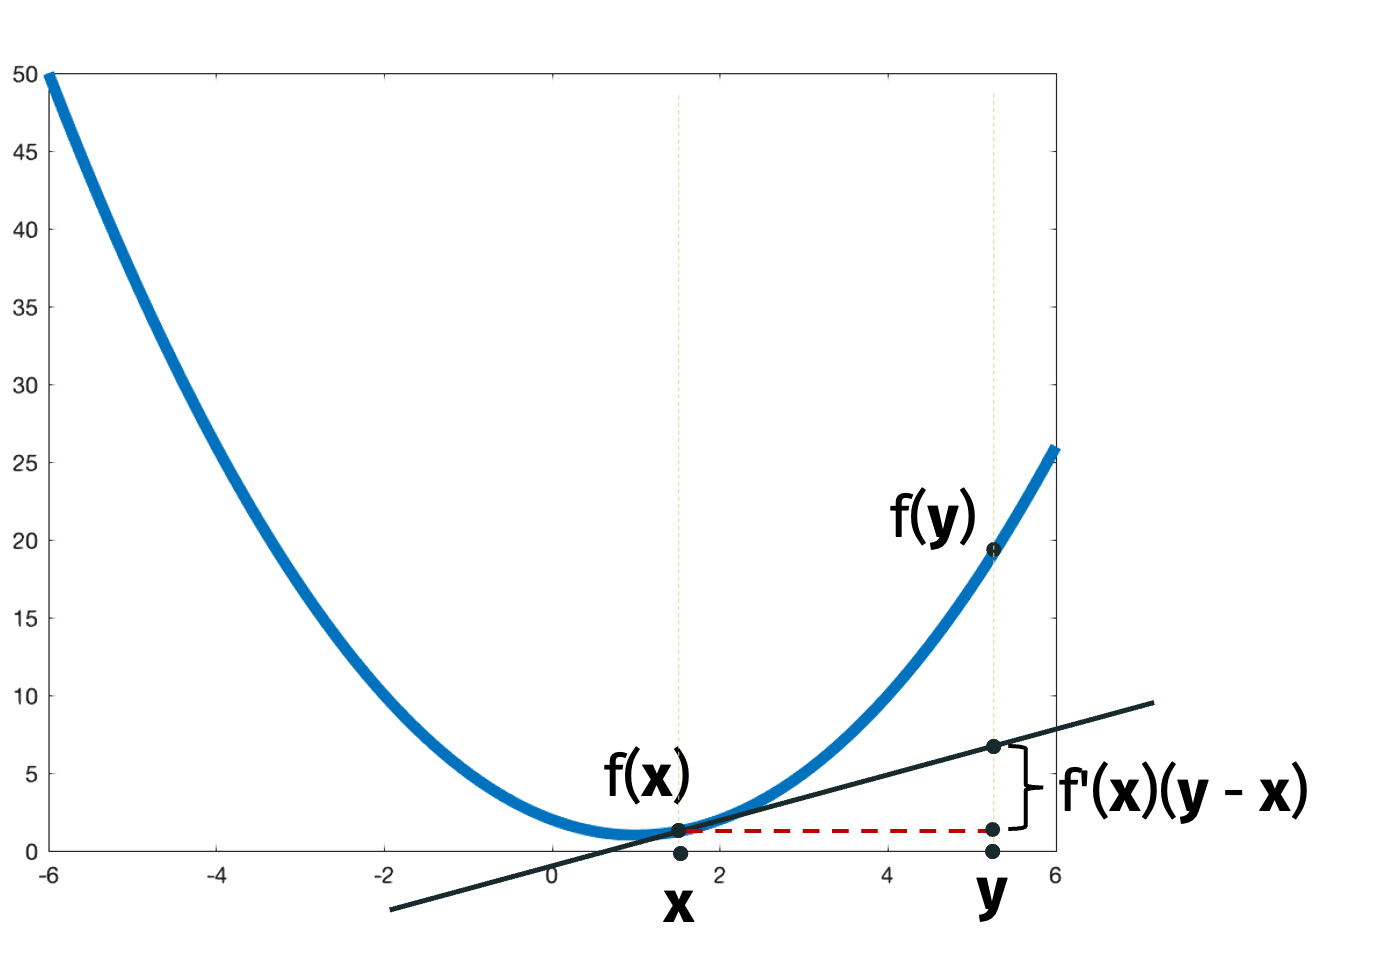
\includegraphics[width=.6\textwidth]{first_second_cond.png}

		\textbf{Recall:} For all convex functions $[f(y) - f(x)] - f'(x)(y-x) \geq 0$. 
	\end{center}
 \end{frame}

 \begin{frame}[t]
	\frametitle{second order conditions}
	Proof that $f''(x)\leq \beta \Rightarrow [f(y) - f(x)] - f'(x)(y-x) \leq \frac{\beta}{2}(y-x)^2$:

	\vspace{15em} Proof for $\alpha$-strongly convex is similar, as are the other directions. 
 \end{frame}

 \begin{frame}[t]
	\frametitle{multidimensional generalization}
	A function is \alert{ $\alpha$-strongly convex} and \alert{$\beta$-smooth} if for all $\bv{x}$, $\bv{y}$:
	\begin{align*}
		\frac{\alpha}{2}\|\bv{y} - \bv{x}\|_2^2 \leq \left[f(\bv{y}) - f(\bv{x})\right] - \nabla f(\bv{x})^T(\bv{y} - \bv{x}) \leq \frac{\beta}{2}\|\bv{y}-\bv{x}\|_2^2
	\end{align*}
\vspace{-2em}
\begin{center}
	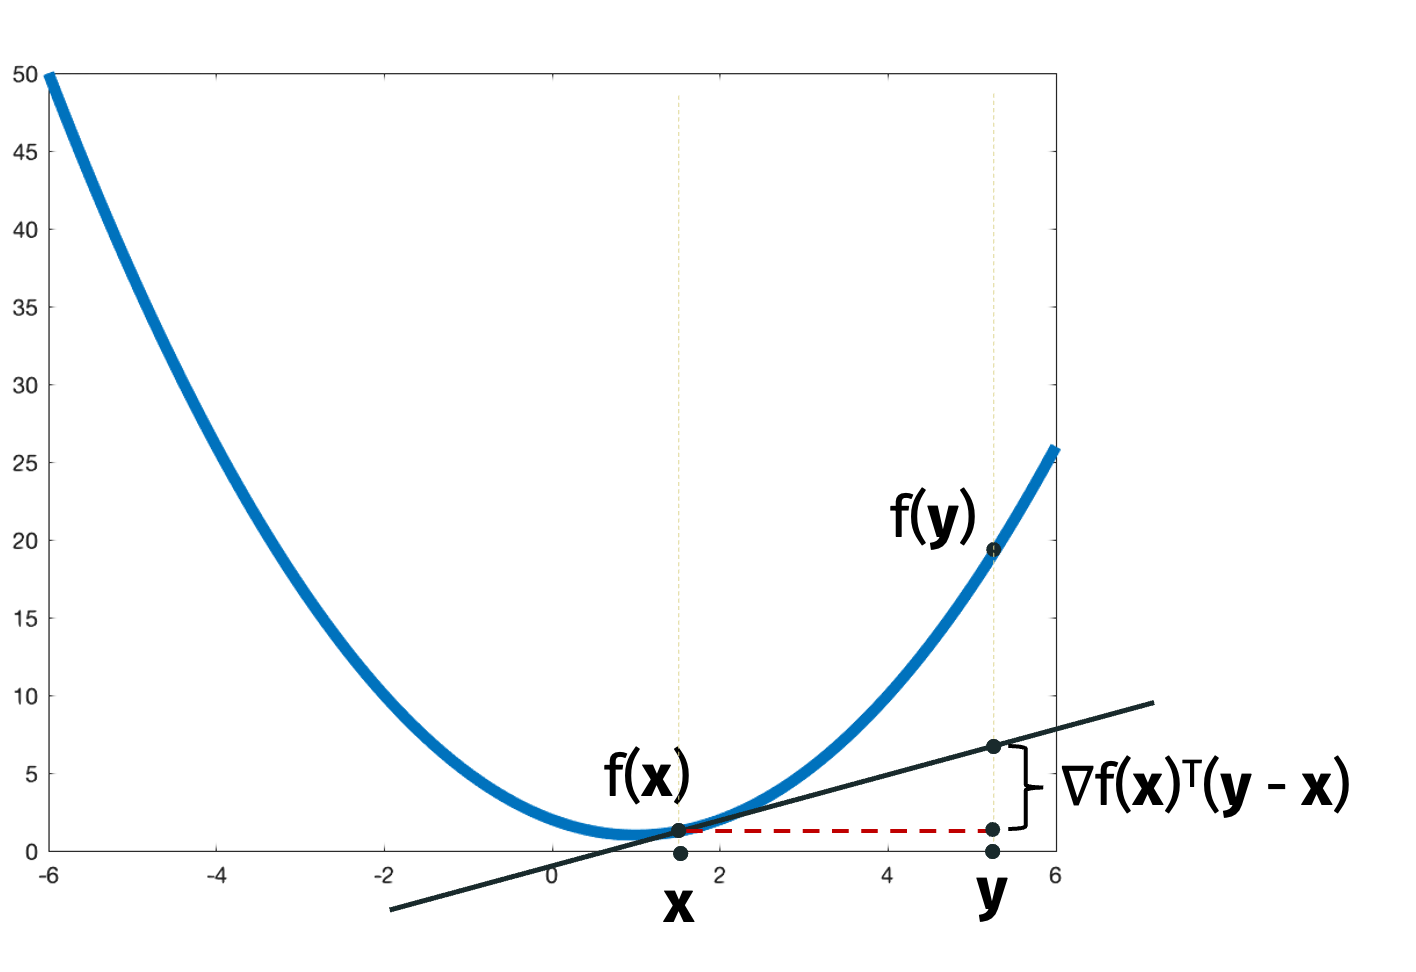
\includegraphics[width=.75\textwidth]{smoothness_image.png}
\end{center}	
\end{frame}


\begin{frame}[t]
	\frametitle{alernative definition of smoothness}
	\begin{definition}[$\beta$-smoothness]
		A function $f$ is $\alert{\beta}$ smooth if and only if, for all $\bv{x}$, $\bv{y}$
		\begin{align*}
			\|\nabla f(\bv{x}) - \nabla f(\bv{y})\|_2 \leq \alert{\beta} \|\bv{x} - \bv{y}\|_2
		\end{align*}
	\end{definition}
	I.e., the gradient function is a \emph{$\beta$-Lipschitz function.} 
	
	We won't use this definition directly, but it's good to know. Easy to prove equivalency to previous definition (see Lem. 3.4 in \color{blue}\textbf{\href{https://arxiv.org/pdf/1405.4980.pdf}{Bubeck's book}}\color{black}).
 \end{frame}

% \begin{frame}[t]
% 	\frametitle{smoothness}
% 	Recall from convexity that $f(\bv{y}) - f(\bv{x}) \geq \nabla f(\bv{x})^T(\bv{y} - \bv{x})$.
% 	\begin{center}
% 		\alert{So now we have an upper and lower bound.}
% 	\end{center}
% \vspace{-1em}
% 	\begin{align*}
% 		0 \leq \left[f(\bv{y}) - f(\bv{x})\right] - \nabla f(\bv{x})^T(\bv{y} - \bv{x}) \leq \frac{\beta}{2}\|\bv{x} - \bv{y}\|_2^2
% 	\end{align*}
% \vspace{-2em}
% \begin{center}
% 	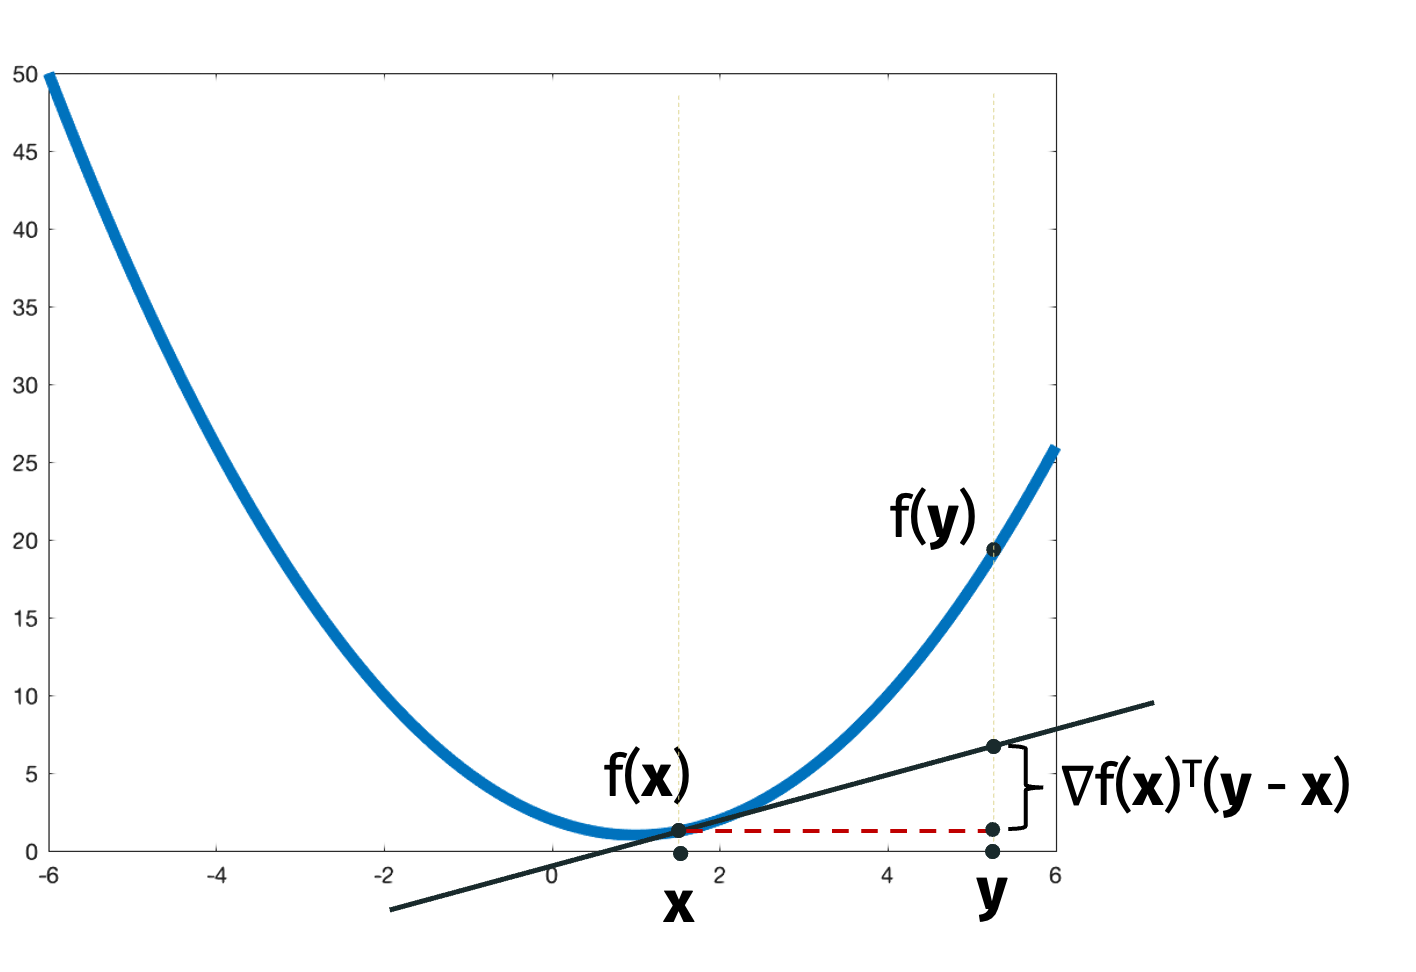
\includegraphics[width=.75\textwidth]{smoothness_image.png}
% \end{center}	
% \end{frame}

\begin{frame}[t]
	\frametitle{convergence guarantee}
	\begin{theorem}[GD convergence for $\beta$-smooth functions.]
		Let $f$ be a \alert{$\beta$} smooth convex function and assume we have $\|\bv{x}^{*} - \bv{x}^{(0)}\|_2 \leq \alert{R}$. If we run GD for $T$ steps, we have:
		\begin{align*}
			f(\bv{x}^{(T)}) - f(\bv{x}^*) \leq \frac{2\beta R^2}{T} 
		\end{align*} 
	\end{theorem}
	\textbf{Corollary}: If \alert{$T = O\left(\frac{\beta R^2}{\epsilon}\right)$} we have $f(\bv{x}^{(T)}) - f(\bv{x}^*) \leq \epsilon$.
	
	\vspace{1em}
		Compare this to $T = O\left(\frac{G^2 R^2}{\epsilon^2}\right)$ without  a smoothness assumption.
\end{frame}

\begin{frame}[t]
	\frametitle{guaranteed progress}
	\begin{center}
	Why do you think gradient descent might be faster when a function is $\beta$-smooth?
	\end{center}
\end{frame}

\begin{frame}[t]
	\frametitle{guaranteed progress}
	Previously learning rate/step size $\eta$ depended on $G$. Now choose it based on $\beta$:\vspace{-.75em}
	\begin{align*}
		\bv{x}^{(t+1)} \leftarrow \bv{x}^{(t)} - \frac{1}{\beta}\nabla f(\bv{x}^{(t)})
	\end{align*}
	
	\textbf{Progress per step of gradient descent:}
	\begin{enumerate}[1.]
		\item $\left[f(\bv{x}^{(t+1)}) - f(\bv{x}^{(t)})\right] - \nabla f(\bv{x}^{(t)})^T(\bv{x}^{(t+1)} - \bv{x}^{(t)})  \leq \frac{\beta}{2}\|\bv{x}^{(t)} - \bv{x}^{(t+1)}\|_2^2.$\vspace{3em}
		\item $\left[f(\bv{x}^{(t+1)}) - f(\bv{x}^{(t)})\right] + 
		\frac{1}{\beta}\|\nabla f(\bv{x}^{(t)})\|_2^2 \leq \frac{\beta}{2}\|\frac{1}{\beta}\nabla f(\bv{x}^{(t)})\|_2^2.$\vspace{3em}
		\item $f(\bv{x}^{(t)}) - f(\bv{x}^{(t+1)}) \geq \alert{\frac{1}{2\beta}\|\nabla f(\bv{x}^{(t)})\|_2^2}.$
	\end{enumerate}
%	\begin{align*}
%		\left[f(\bv{x}^{(t+1)}) - f(\bv{x}^{(t)})\right] - \nabla f(\bv{x}^{(t)})^T(\bv{x}^{(t+1)} - \bv{x}^{(t)})  \leq \frac{\beta}{2}\|\bv{x}^{(t)} - \bv{x}^{(t+1)}\|_2^2\\
%	\end{align*}
%	\begin{align*}
%		\left[f(\bv{x}^{(t+1)}) - f(\bv{x}^{(t)})\right] + 
%		\frac{1}{\beta}\|\nabla f(\bv{x}^{(t)})\|_2^2 \leq \frac{\beta}{2}\|\frac{1}{\beta}\nabla f(\bv{x}^{(t)})\|_2^2 \\
%	\end{align*}
%	\begin{align*}
%		f(\bv{x}^{(t)}) - f(\bv{x}^{(t+1)}) \geq \alert{\frac{1}{2\beta}\|\nabla f(\bv{x}^{(t)})\|_2^2}.
%	\end{align*}
\end{frame}

%\begin{frame}[t]
%	\frametitle{telescoping sum}
%	\textbf{Claim:} For all $t$, $f(\bv{x}^{(t)}) - f(\bv{x}^{(t+1)}) \geq \alert{\frac{1}{2\beta}\|\nabla f(\bv{x}^{(t)})\|_2^2}.$
%	
%	\begin{align*}
%		f(x^{(0)}) - f(x^{(T)}) \geq \frac{1}{2\beta} \sum_{t=0}^T\|\nabla f(\bv{x}^{(t)})\|_2^2
%	\end{align*}
%	
%\end{frame}


\begin{frame}[t]
	\frametitle{convergence guarantee}
	Once we have the bound from the previous page, proving a convergence result isn't hard, but not obvious. A concise proof can be found in Page 15 in \textcolor{blue}{\href{https://gowerrobert.github.io/pdf/M2_statistique_optimisation/grad_conv.pdf}{Garrigos and Gower's notes}.}
	\vspace{.5em}

	\begin{theorem}[GD convergence for $\beta$-smooth functions.]
		Let $f$ be a \alert{$\beta$} smooth convex function and assume we have $\|\bv{x}^{*} - \bv{x}^{(1)}\|_2 \leq \alert{R}$. If we run GD for $T$ steps with $\eta = \frac{1}{\beta}$ we have:
		\begin{align*}
			f(\bv{x}^{(T)}) - f(\bv{x}^*) \leq \frac{2\beta R^2}{T} 
		\end{align*} 
	\end{theorem}
	\textbf{Corollary}: If \alert{$T = O\left(\frac{\beta R^2}{\epsilon}\right)$} we have $f(\bv{x}^{(T)}) - f(\bv{x}^*) \leq \epsilon$.
\end{frame}

\begin{frame}[t]
	\frametitle{guaranteed progress}
	\begin{center}
		Where did we use convexity in this proof?
	\end{center}
	
	\textbf{Progress per step of gradient descent:}
	\begin{enumerate}[1.]
		\item $\left[f(\bv{x}^{(t+1)}) - f(\bv{x}^{(t)})\right] - \nabla f(\bv{x}^{(t)})^T(\bv{x}^{(t+1)} - \bv{x}^{(t)})  \leq \frac{\beta}{2}\|\bv{x}^{(t)} - \bv{x}^{(t+1)}\|_2^2.$\vspace{1.5em}
		\item $\left[f(\bv{x}^{(t+1)}) - f(\bv{x}^{(t)})\right] + 
		\frac{1}{\beta}\|\nabla f(\bv{x}^{(t)})\|_2^2 \leq \frac{\beta}{2}\|\frac{1}{\beta}\nabla f(\bv{x}^{(t)})\|_2^2.$\vspace{1.5em}
		\item $f(\bv{x}^{(t)}) - f(\bv{x}^{(t+1)}) \geq {\frac{1}{2\beta}\|\nabla f(\bv{x}^{(t)})\|_2^2}.$
	\end{enumerate}
\end{frame}

\begin{frame}[t]
	\frametitle{stationary points}
	\begin{definition}[Stationary point]
		For a differentiable function $f$, a \emph{stationary point} is any $\bv{x}$ with: 
		\begin{align*}
			\nabla f(\bv{x}) = \bv{0}
		\end{align*}
	\end{definition}
	\begin{center}
		local/global minima - local/global maxima - saddle points
	\end{center}
\end{frame}

\begin{frame}[t]
	\frametitle{convergence to stationary point}
	\begin{theorem}[Convergence to Stationary Point]
	For \emph{any} $\beta$-smooth differentiable function $f$ (convex or not), if we run GD for $T$ steps, we can find a point $\hat{\bv{x}}$ such that:
	\begin{align*}
		\|\nabla f(\hat{\bv{x}})\|_2^2 \leq  \frac{2\beta}{T} \left( f(\bv{x}^{(0)}) -  f(\bv{x}^{*})\right)
	\end{align*} 
\end{theorem}
\textbf{Corollary:} If $T \geq \frac{2\beta}{\epsilon}$, then $\|\nabla f(\hat{\bv{x}})\|_2^2 \leq \epsilon  \left( f(\bv{x}^{(0)}) -  f(\bv{x}^{*})\right)$.
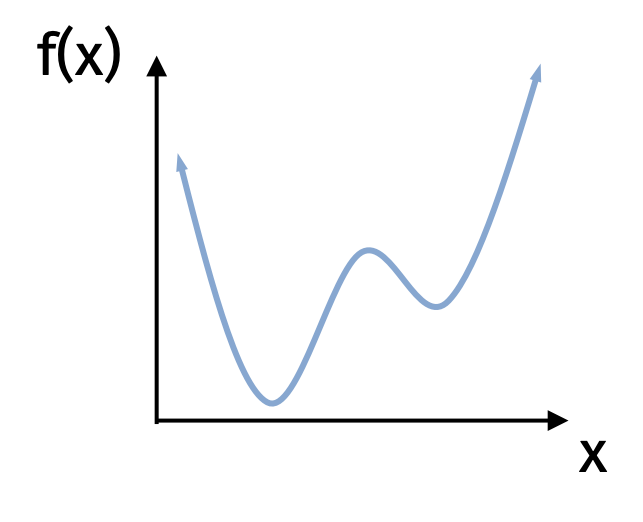
\includegraphics[width=.4\textwidth]{simple_non_convex.png}
\end{frame}

\begin{frame}[t]
	\frametitle{telescoping sum proof}
	\begin{theorem}[Convergence to Stationary Point]
		For \emph{any} $\beta$-smooth differentiable function $f$ (convex or not), if we run GD for $T$ steps, we can find a point $\hat{\bv{x}}$ such that:
		\begin{align*}
			\|\nabla f(\hat{\bv{x}})\|_2^2 \leq  \frac{2\beta}{T} \left( f(\bv{x}^{(0)}) -  f(\bv{x}^{*})\right) 
		\end{align*} 
	\end{theorem}
We have that $\frac{1}{2\beta}\|\nabla f(\bv{x}^{(t)})\|_2^2 \leq f(\bv{x}^{(t)}) - f(\bv{x}^{(t+1)}).$ So: 
\begin{align*}
	\sum_{t=0}^{T-1}\frac{1}{2\beta}\|\nabla f(\bv{x}^{(t)})\|_2^2 &\leq f(\bv{x}^{(0)}) -  f(\bv{x}^{(t)})\\
	\frac{1}{T}\sum_{t=0}^{T-1}\|\nabla f(\bv{x}^{(t)})\|_2^2 &\leq \frac{2\beta}{T} \left( f(\bv{x}^{(0)}) -  f(\bv{x}^{*})\right)\\
	\min_t \|\nabla f(\bv{x}^{(t)})\|_2^2 &\leq \frac{2\beta}{T} \left( f(\bv{x}^{(0)}) -  f(\bv{x}^{*})\right)
\end{align*}
\end{frame}

\begin{frame}[t]
	\frametitle{back to convex functions}
	I said it was a bit tricky to prove that $f(\hat{\bv{x}}) - f(\bv{x}^*) \leq \frac{2\beta R^2}{T}$ for convex functions. But we just easily proved that $\|\nabla f(\hat{\bv{x}})\|_2^2$ is small. Why doesn't this show we are close to the minimum?
	
\end{frame}

\begin{frame}[t]
	\frametitle{strong convexity}
	\begin{definition}[$\alpha$-strongly convex]
		A convex function $f$ is $\alert{\alpha}$-strongly convex if, for all $\bv{x}$, $\bv{y}$
		\begin{align*}
			\left[f(\bv{y}) - f(\bv{x})\right] - \nabla f(\bv{x})^T(\bv{y} - \bv{x}) \geq \frac{\alpha}{2}\|\bv{x} - \bv{y}\|_2^2 
		\end{align*}
	\end{definition}
	Compare to smoothness condition.
	$$\left[f(\bv{y}) - f(\bv{x})\right] - \nabla f(\bv{x})^T(\bv{y} - \bv{x}) \leq \alert{\frac{\beta}{2}}\|\bv{x} - \bv{y}\|_2^2.$$
	
	\vspace{1em}
	For a twice-differentiable scalar function $f$, equivalent to $f''(x) \geq \alpha$.  
	
	\vspace{1em}
	When $f$ is convex, we always have that $f''(x)\geq 0$, so larger values of $\alpha$ correspond to a ``stronger'' condition.
\end{frame}



\begin{frame}[t]
	\frametitle{gd for strongly convex function}
	\textbf{Gradient descent for strongly convex functions:}
	\begin{itemize}
		\item Choose number of steps $T$.
		\item For $i = 0,\ldots, T$:
		\begin{itemize}
			\item $\eta = \frac{2}{\alpha\cdot(i+1)}$
			\item $\bv{x}^{(i+1)} = \bv{x}^{(i)} - \eta \nabla f(\bv{x}^{(i)})$
		\end{itemize}
		\item Return $\hat{\bv{x}} = \argmin_{\bv{x}^{(i)}} f(\bv{x}^{(i)})$. 
		%		\item Alternatively, return $\hat{\bv{x}} = \sum_{i=1}^T \frac{2i}{T(T+1)} \bv{x}^{(i)}$.
	\end{itemize}
\end{frame}

\begin{frame}[t]
	\frametitle{convergence guarantee}
	\begin{theorem}[GD convergence for $\alpha$-strongly convex functions.]
		Let $f$ be an \alert{$\alpha$}-strongly convex function and assume we have that, for all $\bv{x}$, $\|\nabla f(\bv{x})\|_2 \leq \alert{G}$. If we run GD for $T$ steps (with adaptive step sizes) we have:
		\begin{align*}
			f(\hat{\bv{x}}) - f(\bv{x}^*) \leq \frac{2G^2}{\alpha T} 
		\end{align*} 
	\end{theorem}
	\textbf{Corollary}: If \alert{$T = O\left(\frac{G^2}{\alpha \epsilon}\right)$} we have $f(\hat{\bv{x}}) - f(\bv{x}^*) \leq \epsilon$
\end{frame}


\begin{frame}[t]
	\frametitle{convergence guarantee}
	We could also have that $f$ is both $\beta$-smooth and $\alpha$-strongly convex.
	
	\begin{theorem}[GD for $\beta$-smooth, $\alpha$-strongly convex.]
		Let $f$ be a $\beta$-smooth and $\alpha$-strongly convex function. If we run GD for $T$ steps (with step size $\eta = \frac{1}{\beta}$) we have:
		\begin{align*}
			\|\bv{x}^{(T)} - \bv{x}^*\|_2^2 \leq e^{-T \frac{\alpha}{\beta}} \|\bv{x}^{(0)} - \bv{x}^*\|_2^2
		\end{align*} 
	\end{theorem}	
	\begin{center}
		\alert{$\kappa = \frac{\beta}{\alpha}$} is called the ``condition number'' of $f$. 
		
		\textbf{Is it better if $\kappa$ is large or small?}
	\end{center}
\end{frame}

% \begin{frame}[t]
% 	\frametitle{smooth and strongly convex}
% 	\textbf{Converting to more familiar form:}
% 	Using that fact the $\nabla f(\bv{x}^*) = \bv{0}$ along with
% 	\begin{align*}
% 		{\frac{\alpha}{2}}\|\bv{x} - \bv{y}\|_2^2 \leq  \left[f(\bv{y}) - f(\bv{x})\right] - \nabla f(\bv{x})^T(\bv{y} - \bv{x}) \leq {\frac{\beta}{2}}\|\bv{x} - \bv{y}\|_2^2, 
% 	\end{align*}
% 	we have:
% 	\begin{align*}
% 		\|\bv{x}^{(0)} - \bv{x}^*\|_2^2 &\leq \frac{2}{\alpha} \left[f(\bv{x}^{(0)}) - f(\bv{x}^*)\right]\\
% 		\|\bv{x}^{(T)} - \bv{x}^*\|_2^2 &\geq \frac{2}{\beta} \left[f(\bv{x}^{(T)}) - f(\bv{x}^*)\right]
% 	\end{align*}	
% \end{frame}

\begin{frame}[t]
	\frametitle{smooth and strongly convex}
	\textbf{Converting to more familiar form:}
	Using that fact the $\nabla f(\bv{x}^*) = \bv{0}$ along with
	\begin{align*}
		{\frac{\alpha}{2}}\|\bv{x} - \bv{y}\|_2^2 \leq  \left[f(\bv{y}) - f(\bv{x})\right] - \nabla f(\bv{x})^T(\bv{y} - \bv{x}) \leq {\frac{\beta}{2}}\|\bv{x} - \bv{y}\|_2^2, 
	\end{align*}
	we have:
	\begin{align*}
		\|\bv{x}^{(T)} - \bv{x}^*\|_2^2 &\geq \frac{2}{\beta} \left[f(\bv{x}^{(T)}) - f(\bv{x}^*)\right].
	\end{align*}	
We also assume
\begin{align*}
			\|\bv{x}^{(0)} - \bv{x}^*\|_2^2 &\leq R^2.
\end{align*}
\end{frame}

\begin{frame}[t]
	\frametitle{convergence guarantee}
	\begin{corollary}[GD for $\beta$-smooth, $\alpha$-strongly convex.]
		Let $f$ be a $\beta$-smooth and $\alpha$-strongly convex function. If we run GD for $T$ steps (with step size $\eta = \frac{1}{\beta}$) we have:
		\begin{align*}
			f(\bv{x}^{(T)}) - f(\bv{x}^*)  \leq \frac{\beta}{2} e^{-T\frac{\alpha}{\beta}} \cdot  R^2
		\end{align*} 
	\end{corollary}	
	\textbf{Corollary}: 
	If \alert{$T = O\left(\frac{\beta}{\alpha}\log(R\beta/\epsilon)\right)$} we have:
	\begin{align*}
		f({\bv{x}}^{(T)}) - f(\bv{x}^*) \leq \epsilon
	\end{align*}
	Only depend on $\log(1/\epsilon)$ instead of on $1/\epsilon$ or $1/\epsilon^2$!
\end{frame}

\begin{frame}{title}
	\frametitle{smooth, strongly convex optimization}
	We are going to prove the guarantee on the previous page for the special case of:
	\begin{align*}
		f(\bv{x}) = \frac{1}{2}\|\bv{A}\bv{x} - \bv{b}\|_2^2
	\end{align*}
	\textbf{Goal:} Get some of the key ideas across, introduces important concepts like the Hessian, and show the connection between conditioning and linear algebra.
	
\end{frame}



\end{document} 








